%%%%    !!!!!!!!!!!!!!!!!!!!!
%%%%    DŮLEŽITÉ
%%%%
%%%%    Před generováním finální verze spusť nad souborem program vlna
%%%%    http://www.fit.vutbr.cz/~martinek/latex/czech.html
%%%%    Ten zajistí, aby řádek nekončil samostatným znakem a, i, o apod.
%%%%
%%%%    !!!!!!!!!!!!!!!!!!!!!






\documentclass[
  digital,
  twoside,
  table, 
  nolof, 
  nolot
]{fithesis3}

\usepackage[resetfonts]{cmap} 
\usepackage[T1,T2A]{fontenc} 
\usepackage{epsfig}
\usepackage{verbatim}
\usepackage{hyperref}

\usepackage[
  main=czech
]{babel}

\usepackage{paratype}
\def\textrussian#1{{\usefont{T2A}{PTSerif-TLF}{m}{rm}#1}}

\thesissetup{
    date          = \the\year/\the\month/\the\day,
    university    = mu,
    faculty       = fi,
    type          = bc,
    author        = {Jan Laštůvka},
    gender        = m,
    advisor       = {RNDr. Jan Vykopal, Ph.D.},
    title         = {Aplikace pro hodnocení kyberbezpečnostního cvičení},
    keywords      = {Kybernetický polygon, obranná bezpečnostní cvičení, CSIRT-MU, KYPO, Python, Django, REST API},
    TeXkeywords   = {Kybernetický polygon, obranná bezpečnostní cvičení, CSIRT-MU, KYPO, Python, Django, REST API},
    abstract      = {V rámci této bakalářské práce byla navržena a~implementována nová aplikace pro hodnocení účastníků kyberbezpečnostního cvičení, která nahradila stávající aplikaci používanou v~prostředí KYPO. V~teoretické části práce je nejdříve představeno cvičení Cyber Czech, kde se tento software používá a~následně je proveden rozbor dříve vytvořené aplikace. Na základě zjištěných nedostatků a~nově definovaných požadavků je navržen datový model a aplikační programové rozhraní. V~rámci praktické části je navržená aplikace implementována za pomocí Django REST Framework a~je zhodnoceno použití aplikace při cvičení Cyber Czech 2018. V~závěru práce jsou stanoveny další doporučení pro rozvoj aplikace.},
    thanks        = {Rád bych poděkovat svému vedoucímu práce RNDr. Janu Vykopalovi, Ph.D. a~dále RNDr. Vítu Rusňákovi, Ph.D. za jejich odborné rady a~pomoc při řešení této práce.},
    bib           = {references-mendeley.bib, bibliography.bib}, 
}
\usepackage{makeidx}      %% The `makeidx` package contains
\makeindex                %% helper commands for index typesetting.
%% These additional packages are used within the document:
\usepackage{paralist} %% Compact list environments
\usepackage{amsmath}  %% Mathematics
\usepackage{amsthm}
\usepackage{amsfonts}
\usepackage{url}      %% Hyperlinks
\usepackage{markdown} %% Lightweight markup
\usepackage{listings} %% Source code highlighting

\lstset{
  basicstyle      = \ttfamily,%
  identifierstyle = \color{black},%
  keywordstyle    = \color{blue},%
  keywordstyle    = {[2]\color{cyan}},%
  keywordstyle    = {[3]\color{olive}},%
  stringstyle     = \color{teal},%
  commentstyle    = \itshape\color{magenta}}
\usepackage{floatrow} %% Putting captions above tables
\floatsetup[table]{capposition=top}

\begin{document}

\chapter{Úvod}
%\addcontentsline{toc}{chapter}{Úvod}

Žijeme v~digitalizované době, kdy se internet stal součástí života více než jedné poloviny populace \cite{worldStats}. Pomocí internetu můžeme přistupovat nejen k~jednoduchým webovým stránkám, ale také k~mnohem komplexnějším informačním systémům. Všechny tyto systémy jsou však v~ohrožení útočníků a~kybernetické útoky, které na tyto systémy cílí, narůstají na intenzitě a~komplexnosti. Z~tohoto důvodu rostou i~nároky kladené na odborníky, kteří se musí postarat o~zabezpečení těch systémů a~musí dokázat reagovat na jakoukoliv formu kybernetického útoku. Jejich znalosti a~zkušenosti jsou rozhodujícím faktorem při prevenci proti útokům, ale také při řešení situací spojených s~probíhajícím útokem.

Vhodnou metodou vzdělávání jsou kybernetická bezpečnostní cvičení, při kterých účastníci soutěží s~ostatními týmy. Prověří si nejen své znalosti a~schopnosti rychle reagovat na hrozící útoky, ale také si například osvojí vedení komunikace s~médii nebo orgány činnými v~trestním řízení. Jedním z~těchto cvičení je i~Cyber Czech, které je prozatím jediné pravidelně pořádané cvičení svého druhu v~České republice \cite{cyberex}. Akce probíhá v~Kybernetickém polygonu Masarykovy univerzity, který vznikl v~roce 2015 a~nabízí technické prostředky pro vytvoření plně funkčních počítačových sítí a~zařízení ve virtuálním prostředí.

Předmětem této práce je inovace aplikace, která slouží k~hodnocení účastníků cvičení Cyber Czech a~k~prezentaci výsledků z~tohoto cvičení. Během používání původní aplikace bylo zjištěno, že obsahuje celou řadu nedostatků, nepokrývá všechny požadavky uživatelů a~není navržena tak, aby ji bylo možné snadno rozšiřovat. Z~těchto důvodů a~s~ohledem na další rozvoj aplikace bylo rozhodnuto vyvinout zcela nový systém. 

Nový systém bude rozdělen na dva samostatné celky. Servisní vrstvu, jejíž návrh a~vývoj je předmětem této práce, a~prezentační vrstvu vytvořenou v~rámci jiné práce. Oba tyto celky spolu budou komunikovat díky aplikačnímu programovému rozhraní servisní vrstvy. Výsledná aplikace poskytne uživatelům spolehlivý nástroj, který je nepostradatelnou součástí celého cvičení. 

V kapitole \ref{cyberex} se věnuji popisu samotného cvičení Cyber Czech, jeho organizaci a~významu hodnoticí aplikace. Kapitola \ref{oldApp} popisuje stávající hodnoticí aplikaci a~v~textu jsou podrobně rozebrány veškeré její nedostatky. V~kapitole \ref{newApp} se zabývám návrhem nové hodnoticí aplikace a~v~následující kapitole \ref{implementationNewApp} se zaměřuji na samotnou implementaci nové aplikace a~popisuji problémy, se kterými jsem se při vývoji zabýval. V~závěrečné kapitole \ref{end} shrnuji dosažené cíle mojí práce a~formuluji doporučení pro další vývoj celého systému.

\chapter{Kyberbezpečnostní cvičení Cyber Czech}
\label{cyberex}

Pro kyberbezpečnostní profesionály jsou nezbytné znalosti nejrůznějších typů útoků a~způsoby, jak se proti těmto útokům bránit. Z~tohoto důvodu se stávají stále populárnější kyberbezpečnostní cvičení, kde mohou účastníci nové znalosti a~zkušenosti získávat a~prohlubovat pomocí aktivního zapojení do cvičení.

V následující kapitole popisuji Kybernetický polygon Masarykovy univerzity a~kyberbezpečnostní cvičení Cyber Czech, které je zde pořádáno. Věnuji se popisu účastníků tohoto cvičení a~představení systému hodnocení, včetně hodnoticí aplikace.

\section{Kybernetický polygon Masarykovy univerzity}

Kybernetický polygon Masarykovy univerzity (zkráceně KYPO) vznikl jako projekt s~unikátním prostředím uzpůsobeným pro výzkum, vývoj a~analýzu hrozeb v~oboru informační bezpečnosti a~bezpečnosti kritických informačních infrastruktur. Provádí se v~něm školení a~cvičení počítačové bezpečnosti, výzkum ochrany proti kybernetickým útokům, forenzní analýzy a~bezpečnostní experimenty nad počítačovými sítěmi.

KYPO je navržen jako modulární distribuovaný systém \cite{Vykopal2017KYPOCases}. Virtuální prostředí KYPO je vytvořeno v~cloudu, ve kterém je možné velice rychle a~opakovaně vytvářet nové funkční počítačové sítě včetně zařízení v~nich. Stejně tak je možné velice snadno provádět údržbu těchto sítí a~zařízení. Uzavřené virtuální prostředí KYPO zajišťuje, aby uživatelé mohli ve vytvořených sítích bezpečně provádět jakékoliv experimenty, aniž by mohly být ovlivněny počítačové systémy mimo toto prostředí.

KYPO slouží pro výuku studentů Masarykovy univerzity a~kromě již zmíněného kyberbezpečnostního cvičení Cyber Czech zde probíhají i~jiné vzdělávací akce. Jednou z těchto akcí jsou například CTF (Capture the Flag) hry, které jsou zaměřeny na výuku základních technik penetračního testování počítačových sítí a~jejich služeb. Účastník hry se nachází v~roli útočníka, který postupuje několika úrovněmi hry a~jeho hlavním cílem je převzít kontrolu nad serverem a~využít jej pro následný DDoS útok \cite{Vykopal2017KYPOCases}.

\section{Popis cvičení Cyber Czech}

Cyber Czech je kyberbezpečnostní cvičení, pořádané od roku 2015 Masarykovou univerzitou spolu s~Národním centrem kybernetické bezpečnosti, který je součástí Národního bezpečnostního úřadu. Jedná se o~cvičení, které je postaveno na principu, kdy proti sobě stojí dva týmy, tým modrý (bránící) a~tým červený (útočící). Cílem červeného týmu je napadnout různé systémy ve virtuální infrastruktuře modrého týmu, který se naopak snaží proti těmto útokům ubránit.

Během cvičení jsou ověřovány technické znalosti členů modrého týmu, ale zároveň jsou zkoušeny i~jejich schopnosti jednání ve stresových situacích a~v~časové tísni. Kromě technických dovedností musejí členové modrých týmů například zvládat komunikovat s~fiktivními novináři, policií nebo legitimními uživateli jejich systému.

Jedná se o~cvičení, zahrnující aktivní formu účasti, které je určeno odborníkům z~řad správců počítačových systémů. Cvičení je postaveno především na principu obrany před útočníky, kteří vykonávají útoky podle předem připraveného scénáře. Útočníci jsou plně seznámeni se síťovou infrastrukturou modrého týmu a~veškerá slabá místa, která útočící tým zneužívá, jsou pečlivě předem připravena.

Celé cvičení je řízeno příběhem, který je všem účastníkům předem představen. Mimo samotný příběh cvičení jsou účastníci předem seznámeni se síťovou infrastrukturou, kterou musí zabezpečovat, a~před samotným zahájením cvičení mají také prostor k~tomu, aby provedli iniciální zabezpečení svěřené sítě.

Cvičení se typicky účastní šest modrých týmů a~každý z~těchto týmů spravuje zcela identickou počítačovou síť. Červený tým na síť každého modrého týmu provádí stejné typy útoků. Celé cvičení probíhá formou soutěže mezi těmito šesti týmy, kdy týmy začínají s~jistým bodovým základem a~během cvičení mohou různými způsoby získávat, nebo naopak ztrácet body. Vítězným týmem je ten, který má na konci cvičení nejvíce bodů. Soutěžní mód cvičení může ovlivňovat hladinu stresu účastníků a~vyvíjet tak napětí a~stres, které jsou přítomny při zvládání reálných situací.

Ke správě skóre modrých týmů během cvičení slouží hodnoticí aplikace, jejíž inovace je předmětem této bakalářské práce. 

\subsection{Účastníci cvičení}
Účastníci cvičení jsou rozděleni do pěti skupin podle jejich úlohy při cvičení. Obrázek \ref{fig:ucastnici} znázorňuje úlohy jednotlivých skupin.

\begin{figure}[ht!]
    \centering
    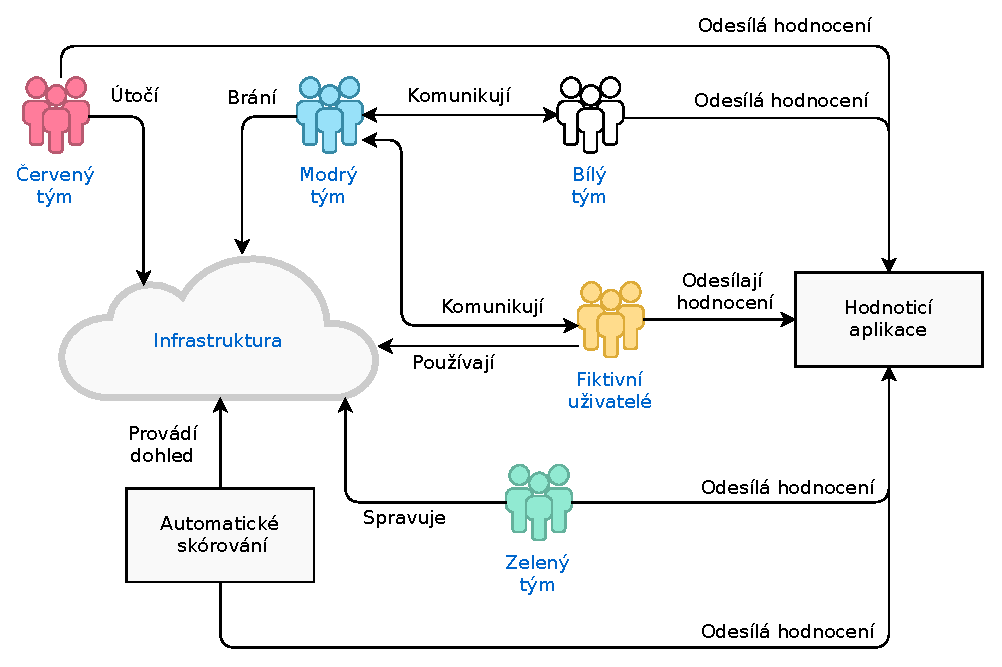
\includegraphics[width=14cm]{images/ucastnici-2.eps}
    \caption{Schéma popisující úlohy jednotlivých skupin účastníků cvičení Cyber Czech.}
    \label{fig:ucastnici}
\end{figure}

\begin{itemize}
\item Modrý tým -- tým hračů, kteří jsou v~průběhu cvičení zkoušeni. Během cvičení se musí řídit pravidly cvičení a~také právními předpisy vztahujícími se na kybernetickou bezpečnost, tedy například ohlašovací povinností kybernetických bezpečnostních incidentů.
\item Červený tým -- tým útočníků, složený z~odborníků na kybernetickou bezpečnost, kteří hodnotí obranné akce modrého týmu. 
\item Bílý tým -- tým lidí, kteří se starají o~organizaci a~průběh cvičení. Dohlížejí na dodržování pravidel cvičení, na vývoj situace mezi červeným týmem a~modrými týmy a~na požádání zodpovídají dotazy modrého týmu. Simulují média, která podle probíhajícího scénáře cvičení vznáší na modré týmy dotazy. Dále simulují právní poradce, orgány činné v~trestním řízení a~jiné fiktivní instituce vystupující ve scénáři.
\item Fiktivní uživatelé -- tým osob, představující reálné uživatele systémů, o~které se modré týmy starají. Provádějí legitimní operace a~modrý tým musí zajistit, aby systémy, se kterými pracují, byly vždy dostupné.
\item Zelený tým -- tým odborníků, spravující celou infrastrukturu používanou na cvičení. Jsou zodpovědní za konfiguraci všech virtuálních počítačů a~sítí, za monitoring sítí a~za skórovací infrastrukturu. Na žádost modrého týmu mohou provést servisní zásah v~jejich síti, typicky obnovení požadovaného stroje do stavu před zahájením cvičení.
\end{itemize}

\subsection{Hodnoticí aplikace}
Pro hodnocení účastníků cvičení Cyber Czech aktuálně slouží na míru vytvořený software, který je dostupný jako webová aplikace a~umožňuje zadávání hodnocení pro modré týmy a~nabízí přehledné zobrazení aktuálního skóre všech modrých týmů. Do programu mají přístup všichni účastníci cvičení, kteří zadávají hodnocení za modré týmy, které do systému přístup nemají. Modré týmy mají pouze přehled prostřednictvím promítání o~svém celkovém skóre a~pořadí mezi týmy. Komplexnější zpětná vazba je účastníkům poskytována až po skončení cvičení \cite{Vykopal2017TimelyExercises}.

\subsection{Hodnocené oblasti}
Během cvičení získávají modré týmy hodnocení, na kterém závisí jejich umístění ve výsledném pořadí. Hodnocení je rozděleno do několika oblastní podle zdroje hodnocení.

\begin{itemize}
\item Hodnocení pomocí automatického skórování -- během cvičení je pomocí automatických systémů kontrolováno, zda v~systému, který modrý tým spravuje, jsou dostupné všechny legitimní služby. Jedná se například o~e-mailové servery, webové služby a~jiné prvky spravovaných systémů. V~případě nedostupnosti uvedených služeb jsou modré týmy adekvátně penalizovány.
\item Hodnocení červeným týmem -- během cvičení provádí červený tým útoky podle předem naplánovaného scénáře. Do hodnoticí aplikace poté červený tým zadává bodovou penalizaci za útoky, které se zdařily.
\item Hodnocení bílým týmem -- bílý tým představuje fiktivní média, orgány činné v~trestním řízení a~zastupuje také roli koordinátora cvičení. Hodnotí převážně intenzitu a~formu komunikace. Bílý tým může zadávat záporné hodnocení za nedostatečnou komunikaci, nebo naopak kladné hodnocení za adekvátní komunikaci.
\item Hodnocení fiktivními uživateli -- při cvičení je nezbytné, aby systémy byly neustále dostupné legitimním uživatelům. V~případě, že systémy nejsou dostupné, případně neumožňují uživatelům plnohodnotné použití, zadává tým fiktivních uživatelů modrému týmu bodovou penalizaci.
\item Hodnocení zeleným týmem -- v~případě, že modrý tým narazí na problémy, které není schopen vyřešit, má možnost si vyžádat servisní zásah od správců infrastruktury. Za každou opravu v~infrastruktuře modrého týmu zelený tým odečte body danému týmu.
\end{itemize}

\subsection{Základní síťová infrastruktura cvičení}
Jak lze vidět na obrázku \ref{fig:kypoNetwork}, síť vytvořená pro potřeby cvičení je rozdělena do dvou podsítí, kterým se budu věnovat v~následujících bodech.

\begin{itemize}
    \item Globální síť -- představuje společnou síťovou infrastrukturu, ve které se nachází např. DNS nebo e-mailové servery. Jedná se o~simulaci veřejného internetu, ve které operují jak útočníci, tak legitimní uživatelé systému. Na serveru v~této síti je spuštěna hodnoticí aplikace, kterou se budu později blíže zabývat. Aby mohli účastníci cvičení například stahovat bezpečnostní aktualizace nebo vyhledávat potřebné informace na webových serverech, je tato síť připojena také k~veřejnému internetu.
    \item Sítě modrých týmů -- každý modrý tým má k~dispozici identickou síť, která je pomocí brány připojena do globální sítě. Každá síť modrého týmu obsahuje kritickou infrastrukturu a~zranitelné služby, které se snaží napadnout červený tým. Síť modrých týmů je dále rozdělena do tří celků -- na demilitarizovanou zónu (DMZ), pracovní stanice a~na servery. V~síti je přítomna monitorovací služba, která sleduje síťový provoz, a~do této služby je integrována logovací infrastruktura. Každý stroj v~síti je poté nakonfigurován tak, aby zapisoval do centrálního logovacího serveru veškeré změny stavu této služby \cite{1319597}. Monitorovací infrastruktury využívá hodnoticí aplikace, která na základě zjištěných nedostupností služeb vytváří bodové penalizace.
\end{itemize}

\begin{figure}[ht]
    \centering
    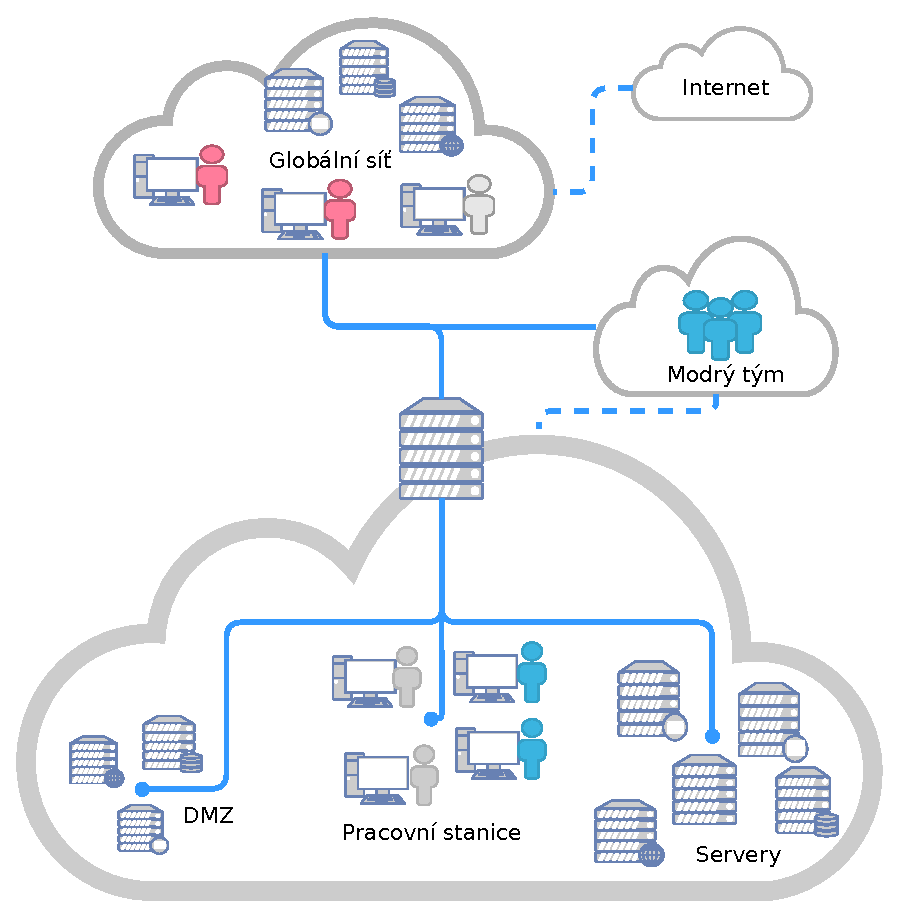
\includegraphics[width=11cm]{images/kypo-network.eps}
    \caption{Schéma rozvržení sítě při kybernetickém cvičení Cyber Czech \cite{Vykopal2017LessonsRange}. Červené piktogramy uživatelů znázorňují, ve které části sítě se nachází útočníci. Šedé piktogramy uživatelů pak označují členy bílého týmu a fiktivních uživatelů. Zbývající modré piktogramy jsou členové modrého týmu.}
    \label{fig:kypoNetwork}
\end{figure}


\chapter{Rozbor původní aplikace}
\label{oldApp}

Původní aplikace pro hodnocení účastníků kyberbezpečnostního cvičení Cyber Czech byla navržena v~rámci diplomové práce \emph{Bezpečnostní cvičení v~prostředí KYPO}, kterou zpracoval Mgr. Milan Kostelník v~roce 2015 \cite{Kostelnik2016thesis}. V~rámci zmíněné diplomové práce byl navržen model hodnocení účastníků cvičení, byly stanoveny funkční požadavky na hodnoticí aplikaci a~dále byl navržen datový model a~základní požadavky na grafické zpracování aplikace. 

Implementace navržené aplikace byla zajištěna Ústavem výpočetní techniky Masarykovy univerzity v~roce 2015. Aplikace byla použita při cvičení Cyber Czech 2015 a~poté v~následujících dvou ročnících tohoto cvičení, díky tomu byly objeveny veškeré nedostatky aplikace a~byl získán dostatek zpětné vazby, jak aplikaci dále rozšířit.

Výsledná implementace aplikace se však v~nejrůznějších detailech lišila od původního návrhu. V~následujícím rozboru proto dále analyzuji vytvořenou aplikaci, popisuji použité technologie a~požadavky na aplikaci a~dále se zaměřuji na její datový model. V~poslední kapitole se podrobně věnuji všem objeveným nedostatkům.

\section{Použité technologie}
Pro implementaci hodnoticí aplikace byl zvolen programovací jazyk Python s~použitím frameworku Django, který je určen pro tvorbu webových systémů. 

Python je dynamicky interpretovaný programovací jazyk. Využívá se pro rychlý vývoj aplikací, které jsou přenositelné na většinu běžných platforem (Unix, Microsoft Windows, macOS). Python lze využít jak pro psaní krátkých skriptů, tak pro vybudování komplexních systémů. Jazyk byl využit ve skriptu pro obsluhu automatického skórování a~zároveň pro vybudování komplexní hodnoticí aplikace. Výhodou je dostupnost velkého množství knihoven, které mohou vývojáři usnadnit rutinní úlohy. Jednou z~těchto knihoven je i~framework Django, pomocí kterého je hodnoticí aplikace vytvořena.

Django je open source webový framework, jehož hlavní úlohou je zjednodušit a~urychlit vývoj komplexních webových aplikací napojených na databázový systém. Tento systém byl zvolen pro svoji jednoduchost a~nabízené výhody. Framework umožňuje snadné budování MVC (Model-view-controller) softwarové architektury, která vede vývojáře k~udržování přehledného a~strukturovaného kódu. Obsahuje propracovaný systém pro objektově relační mapování (ORM), který zajišťuje konverzi dat mezi relační databází a~objektově orientovanou aplikací. Při vývoji je tak programátorovi ulehčena práce s~databázovou vrstvou. Další výhodou je možnost generování automatické administrace pro datový model vytvořený pomocí Django ORM. Framework obsahuje propracovaný systém pro autentizaci a~autorizaci uživatelů. 

\section{Požadavky na hodnoticí aplikaci}

Aby přístup do aplikace byl co nejjednodušší a~zcela nezávislý na operačním systému uživatele, bylo požadováno, aby systém fungoval jako webový portál. Na samotnou aplikace bylo dále stanoveno několik funkčních požadavků \cite{Kostelnik2016thesis}.

\begin{itemize}
\item Kontrola dostupnosti legitimních služeb musí probíhat automaticky a~v~reálném čase.
\item Aplikace bude umožňovat zadání manuálního hodnocení k~událostem, které jsou prováděny červeným týmem, bílým týmem, legitimními uživateli nebo organizátory cvičení.
\item Pro každou událost je nezbytné, aby bylo možné specifikovat dolní a~horní mez bodového ohodnocení.
\item Po odeslání hodnocení bude možné provést jeho opravu, případně zpětné odstranění.
\item Systém umožní provádět správu uživatelů pomocí uživatelských rolí. Uživateli pak bude umožněno odeslat hodnocení pouze za události, které může daný tým hodnotit.
\item Systém umožní zobrazení časomíry pro odpočet času do ukončení cvičení.
\end{itemize}

Funkční požadavky shrnuje diagram případů užití na obr. \ref{fig:useCase1}.

\begin{figure}[ht!]
    \centering
    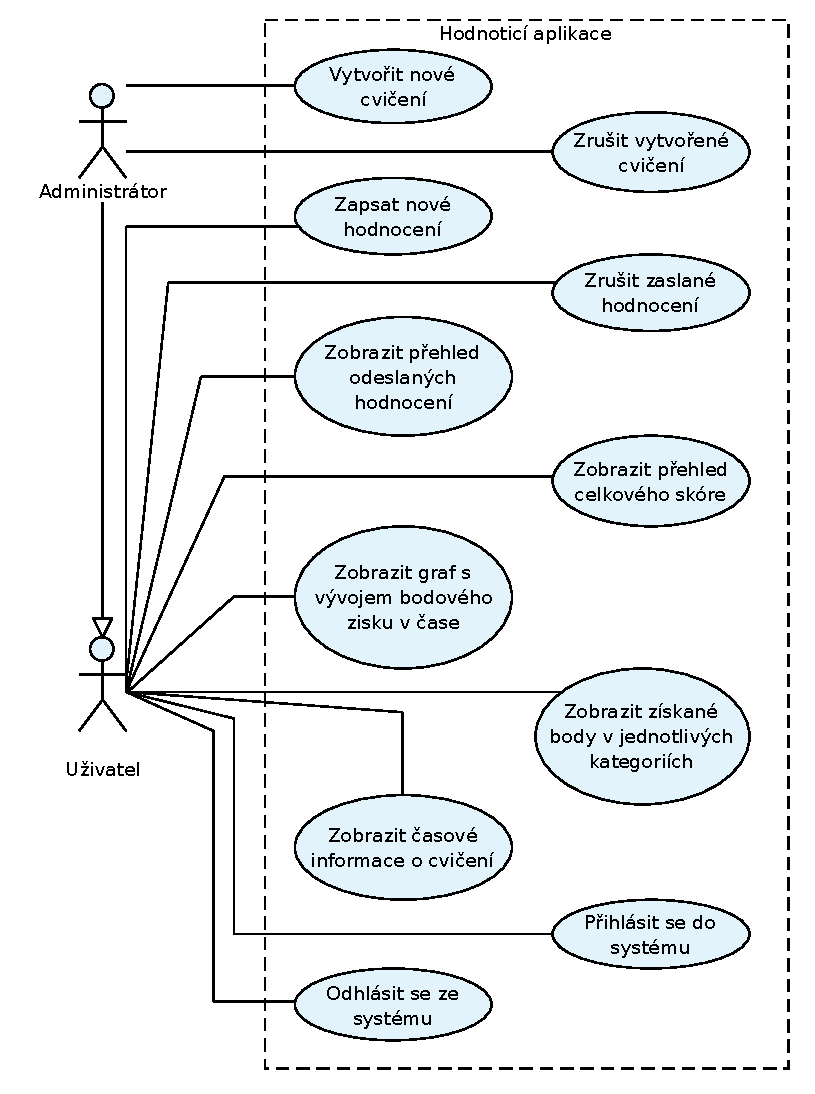
\includegraphics[width=10cm]{images/Use-case-1.eps}
    \caption{Diagram případů užití původní hodnoticí aplikace.}
    \label{fig:useCase1}
\end{figure}

\section{Model hodnocení účastníků cvičení}
Model pro hodnocení týmů, účastnících se cvičení Cyber Czech, byl navržen tak, aby týmy získávaly bodovou penalizaci za nedostupnost předem definovaných služeb (dostupnost byla kontrolována automaticky, proto se používá termín automatické hodnocení) a~dále týmy získávaly, nebo ztrácely body pomocí manuálně zadaného hodnocení od červeného týmu, bílého týmu, fiktivních uživatelů spravovaného systému a~nebo od organizátorů cvičení (zelený tým).

\subsection{Automatické skórování}
Aplikace umožňuje členy modrého týmu bodově penalizovat za nedostupnost legitimních služeb. Pro kontrolu dostupnosti těchto služeb se využívá monitorovací systém přítomný ve virtuálním prostředí KYPO. V~případě nedostupnosti služby je vložen záznam do fronty v~RabbitMQ \cite{rabitmq} serveru a~aplikace si poté tento záznam načte a~vyhodnotí, zda má dojít k~bodové penalizaci daného týmu. Strukturu celého systému automatického hodnocení popisuje obrázek č. \ref{fig:autoScoring}.

\begin{figure}[h!]
    \centering
    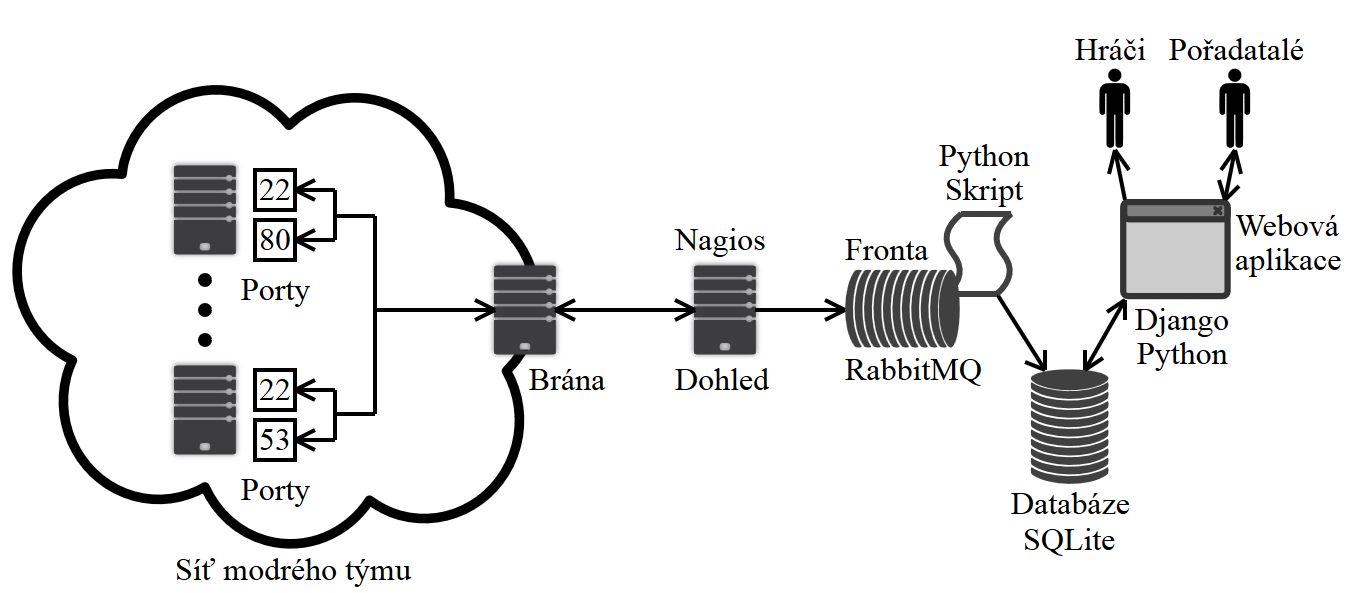
\includegraphics[width=13cm]{images/Page-47-Image-27.png}
    \caption{Struktura systému automatického hodnocení \cite{Kostelnik2016thesis}.}
    \label{fig:autoScoring}
\end{figure}

\subsection{Manuální skórování}
Kromě bodové penalizace za nedostupnost definovaných služeb je v~aplikaci možné zadávat i~manuální bodové ohodnocení. Toto hodnocení zadávají členové červeného týmu, bílého týmu, členové skupiny legitimních uživatelů systému nebo členové zeleného týmu. Zadávat hodnocení je možné jen pro předem definované události, které mají stanovenou dolní a~horní bodovou mez. V~případě červeného týmu odpovídají tyto události předem naplánovaným útokům. Naopak pro bílý tým nebo legitimní uživatele se jedná o~události obecné povahy, např. komunikace s~modrým týmem.

Manuální hodnocení je možné zadávat pomocí formuláře, kde uživatel vybere modrý tým, kterému hodnocení zadává. Dále vybere požadovanou událost, zadá bodové ohodnocení z~definovaného intervalu a~případný slovní komentář. Na obrázku č. \ref{fig:formScore} je ukázka tohoto formuláře, jak byl zpracován v~původní hodnoticí aplikaci.

\begin{figure}[h!]
    \centering
    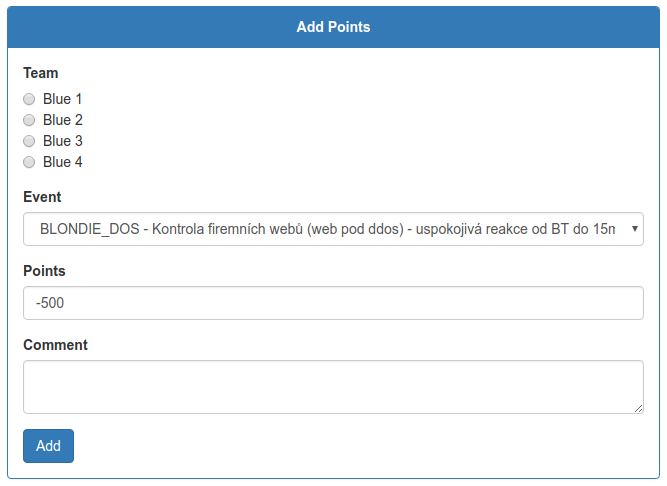
\includegraphics[width=12.8cm]{images/form.png}
    \caption{Snímek obrazovky zachycující formulář pro vložení nového hodnocení v~původní aplikaci.}
    \label{fig:formScore}
\end{figure}

\section{Datový model}
\subsection{Popis datového modelu}

Entitně relační diagram na obr. \ref{fig:erdDjango} ukazuje část systému pro správu uživatelů, která je součástí Django frameworku a~je využívána hodnoticí aplikací. Nyní blíže popíšu entity, které se v~diagramu nachází.

\paragraph{Tabulka \texttt{auth\_user}} Slouží pro ukládání uživatelských účtů. Sloupec \texttt{is\_superuser} označuje super uživatele, který získává nejvyšší oprávnění pro správu systému. Atribut \texttt{is\_staff} identifikuje uživatelský účet, který má přístup do administrace, kterou framework Django automaticky vytváří. Zbývající atribut \texttt{is\_active} reprezentuje, zda je možné se k~účtu přihlásit.

\paragraph{Tabulka \texttt{auth\_group}} Slouží pro ukládání uživatelských skupin, které jsou využity pro rozdělení uživatelů do jednotlivých týmů. 

\paragraph{Tabulka \texttt{auth\_user\_groups}} Zajišťuje vazbu mezi uživateli a~skupinami. Systém pro správu uživatelů dále obsahuje mechanismy pro nastavování oprávnění na úrovni uživatelských skupin. Aplikace však těchto vlastností nevyužívá, a~proto je pro zjednodušení neuvádím.

\begin{figure}[h!]
    \centering
    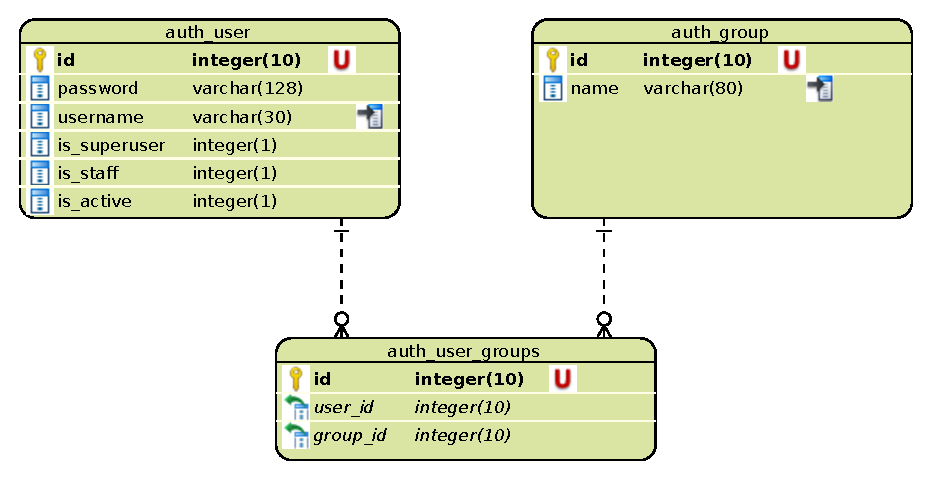
\includegraphics[width=12cm]{images/ERD-django.eps}
    \caption{Entitně relační diagram zachycující strukturu dat v~systému správy uživatelů frameworku Django.}
    \label{fig:erdDjango}
\end{figure}

Při implementaci stávající hodnoticí aplikace byl pozměněn, v diplomové práci, navržený datový model a~vlivem těchto rozdílů se do databáze zanesly nejrůznější nedostatky. V~následujících odstavcích nejdříve popíšu samotný datový model, který je zachycen na obrázku \ref{fig:erdOldApp}. Následně shrnu nedostatky tohoto modelu. 

\begin{figure}[h!]
    \centering
    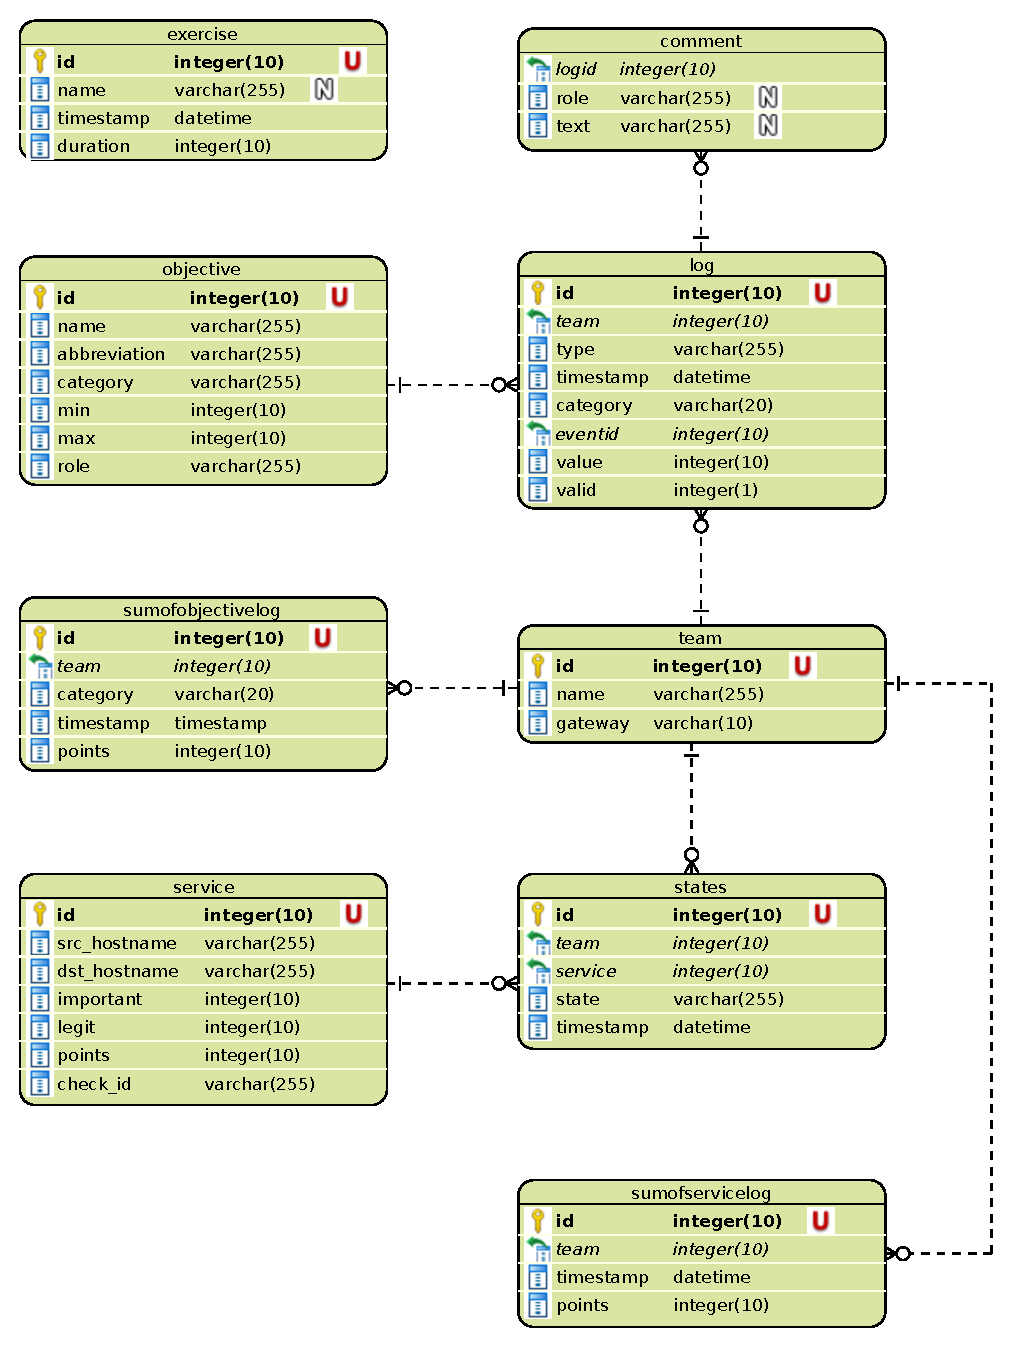
\includegraphics[width=13.5cm]{images/ERD-old-app.eps}
    \caption{Entitně relační diagram popisující datový model původní aplikace.}
    \label{fig:erdOldApp}
\end{figure}

\paragraph{Tabulka \texttt{exercise}} Obsahuje informaci o~vytvořeném cvičení. Do sloupce \texttt{timestamp} se ukládá čas začátku cvičení. Sloupec \texttt{duration} nese informaci o~délce trvání cvičení v~celých hodinách a~do sloupce \texttt{name} je možné z~GUI nastavit hodnotu \texttt{start} nebo \texttt{stop}, která označuje, zda jde o~nastavení času začátku cvičení, nebo ukončení cvičení.

\paragraph{Tabulka \texttt{team}} Obsahuje informace o~týmech účastnících se cvičení. Atribut \texttt{gateway} slouží pro zadání identifikátoru, který identifikuje hodnoty z~automatického skórování pro daný tým.

\paragraph{Tabulka \texttt{objective}} Slouží pro ukládání událostí, za které jsou účastníci cvičení hodnoceni. Pouze na základě akcí, definovaných v~této tabulce, je možné zadávat v~aplikaci bodové ohodnocení soutěžícím týmům. Každá událost má uložen svůj název, zkratku, kategorii, minimální a~maximální bodové ohodnocení a~uživatelskou roli určující, který tým smí hodnocení pro danou událost odeslat. Tento atribut od sebe rozlišuje červený tým, bílý tým, fiktivní uživatele a~nebo je do něj možné uložit hodnotu, která určuje, že danou událost může hodnotit kdokoliv s~přístupem do hodnoticí aplikace.

\paragraph{Tabulka \texttt{log}} Obsahuje záznam o~samotném zadání hodnocení. U~této tabulky došlo k~velkému odchýlení od původního návrhu, protože měla sloužit pro uložení záznamu jak o~automatickém, tak i~manuálním skórování. Výhodou původního záměru mělo být usnadnění sledování skóre v~čase. Avšak ve výsledné implementaci se do této tabulky ukládají data pouze z~manuálního hodnocení. Tabulka obsahuje typ hodnocené události, který je vždy nastaven na hodnotu \texttt{O} a~vazbu na konkrétní tým. Dále časovou značku, kategorii, která odpovídá uživatelské roli uložené pro danou událost v~tabulce \texttt{objective}, referenci na samotnou událost, bodové ohodnocení a~na závěr informaci o~tom, zda je záznam platný. K~tabulce \texttt{log} se dále váže tabulka \texttt{comment}, do které byl uložen případný slovní komentář k~udělenému ohodnocení. Pomocí cizího klíče byla uložena v~tabulce reference na daný záznam.

\paragraph{Tabulka \texttt{sumofobjectivelog}} Účelem této tabulky je snadné zjištění aktuálního skóre daného týmu. Poslední záznam v~této tabulce by měl odpovídat skóre, které tým aktuálně má. To znamená, že tabulka musí být aktualizována s~každou změnou skóre, tedy například i~při smazání chybně zadaného hodnocení. Informace uložená v~této tabulce však může být kdykoliv zjištěna z~tabulky \texttt{log} a~z~tohoto pohledu se tedy jedná o~ukládání duplicitní informace.

\paragraph{Tabulka \texttt{service}} Ukládá seznam služeb, jejíž dostupnost se během cvičení kontroluje pomocí automatického skórování. Tato tabulka obsahuje informaci o~zařízení, na kterém je služba provozována, a~dále port, na kterém by měla být služba dostupná. Atributy \texttt{important} a~\texttt{points} definují, jak velkou bodovou ztrátu týmu způsobí nedostupnost této služby. Sloupec \texttt{legit} označuje, zda jde o~legitimní službu, která musí být dostupná. Pokud sloupec není nastaven na hodnotu 1, není nedostupnost této služby nijak penalizována. 

\paragraph{Tabulka \texttt{states}} Obsahuje záznam o~zkontrolované dostupnosti nebo nedostupnosti dané služby. Při kontrole dané služby je v~tabulce vytvořen záznam, zda je služba, specifikovaná ve sloupci \texttt{service}, dostupná, nebo nedostupná. Stav dostupnosti je uložen v~atributu \texttt{state} pomocí hodnoty \texttt{up} nebo \texttt{down}. Dále se ukládá čas provedené kontroly.

\paragraph{Tabulka \texttt{sumofservicelog}} Jedná se o~tabulku, která je velice podobná tabulce \texttt{sumofobjectivelog} a~je v~ní uložen vývoj skóre z~automatického hodnocení pro každý tým. Poslední vložený záznam pro daný tým by měl odpovídat aktuální hodnotě skóre z~automatického hodnocení.

\subsection{Nedostatky datového modelu}

V původním datovém modelu jsem shledal několik nedostatků. V~následujících odstavcích se zaměřím na ty nejvážnější.

V tabulce \texttt{sumofservicelog} neexistuje žádná vazba, ze které by šlo určit, která služba byla nedostupná a~způsobila tak bodovou penalizaci. Nelze tedy žádným způsobem kontrolovat, která služba stržení bodů způsobila a~nelze ani získat informaci o~tom, kolik bodů bylo celkem za nedostupnost dané služby strženo. V~původním návrhu datového modelu měla být tato informace uložena v~tabulce \texttt{log}, avšak při implementaci se tato tabulka pro automatické hodnocení nevyužila. 

Nelze snadno sledovat vývoj bodového ohodnocení v~čase, protože pro přesné zjištění těchto dat je nutné procházet dvě tabulky (\texttt{log} a~\texttt{sumofservicelog}). Tento nedostatek opět souvisí s~nevyužitím tabulky \texttt{log} i~pro automatické hodnocení.

Tabulky \texttt{sumofservicelog} a~\texttt{sumofobjectivelog} jsou nadbytečné. Data uložená v~těchto tabulkách by bylo možné získat z~tabulky \texttt{log}. Navíc pomocí agregačních dotazů nad touto tabulkou by bylo možné získat celkové skóre v~řádu desítek milisekund i~nad obrovským množstvím záznamů. Nutnost neustálé aktualizace dat v~této tabulce vnáší navíc do aplikace složitější logiku náchylnou na chybu. 

U manuálního hodnocení týmů v~tabulce \texttt{log} dochází k~ukládání reference na tabulku \texttt{objective} a~dále se ukládá i~informace o~uživatelské roli (sloupec \texttt{category}), ze které bylo hodnocení zadáno, avšak tuto informaci je možné zjistit přímo z~vazby na tabulku \texttt{objective}.

V tabulce \texttt{objective} je nadbytečný atribut \texttt{category}, který obsahuje číselný identifikátor role. Sloupec není v~aplikaci nikde využit. Při vytvoření záznamu v~tabulce \texttt{sumofobjectivelog} se tento sloupec překopíruje do sloupce \texttt{category}, ale dále se s~touto hodnotou nikde v~aplikaci nepracuje.

Tabulka \texttt{exercise} umožňuje do sloupce \texttt{name} uložit hodnotu \texttt{start} nebo \texttt{stop}, avšak s~hodnotou \texttt{stop} aplikace žádným způsobem dále nepracuje, jelikož délka cvičení je nastavena atributem \texttt{duration} a~není tedy potřeba nastavovat čas ukončení cvičení. Data v~tabulce \texttt{exercise}, která mají ve sloupci \texttt{name} uloženou hodnotu \texttt{stop}, tedy nemají žádný význam.

V datovém modelu se dále vůbec nepočítalo s~možností ukládat informace o~tom, který uživatel zadal týmu dané hodnocení. Nebylo tedy možné dohledat, kdo je zodpovědný za udělené skóre.

Nedostatkem v~relačním návrhu je skutečnost, že pro ukládání dat, která odpovídají údajům uloženým v~jiné tabulce, není využito cizích klíčů. Např. v~případě uživatelských rolí se ukládá role pouze jako textový název (tabulka \texttt{objective} a~sloupec \texttt{role}). Pro využití klauzule \texttt{JOIN} v~SQL dotazech je toto nevyhovující.

\section{Nedostatky aplikační a~prezentační vrstvy}

Kromě nedostatků v~datovém modelu vykazuje aplikace další anomálie, které se projevují neočekávanými pády aplikace, případně výpisem chybných dat v~aplikaci.

K neočekávanému pádu aplikace dochází např. při odeslání manuálního hodnocení, kde bodové ohodnocení je mimo specifikovaný rozsah. Další chybu způsobovalo odeslání formuláře bez vybraného týmu. Oba případy způsobily pád aplikace, uživateli byla zobrazena chyba a~pomocí tlačítka zpět se musel vrátit na původní stránku.

Chybně se chová i~časomíra, ukazující, kolik času zbývá do konce cvičení. Výpočty s~časem nejsou prováděny správně, a~tak například po ukončení cvičení dojde k~zobrazení časového údaje se záporným počtem hodin, které zbývají do ukončení cvičení.

Aplikace nedisponuje žádným rozhraním pro správu uživatelských účtů, hodnocených událostí (tabulka \texttt{objective}), seznamu služeb (tabulka \texttt{services}) nebo například automatického skóre. Uvedená data je možné upravovat pouze přímým zásahem do databáze.

\chapter{Návrh nové hodnoticí aplikace}
\label{newApp}
Původní hodnoticí aplikace byla použita celkem při třech ročnících cvičení Cyber Czech. Během této doby začaly vznikat nové funkční požadavky na aplikaci, které vyplývaly jak ze zkušeností samotných uživatelů, tak ze zkušeností organizátorů z~řad Masarykovy univerzity a~Národního centra kybernetické bezpečnosti. Vzhledem k~nedostatkům, které původní systém obsahoval, a~nedostatečné modularitě celého systému bylo jako nejvýhodnější řešení zvoleno vytvoření zcela nové aplikace. 

Nová aplikace musí plně zachovat původní funkcionalitu a~být rozšířena o~nové požadavky, ale zároveň musí být opraveny veškeré nedostatky objevené v~původní aplikaci. Z~tohoto důvodu byla nejdříve provedena revize datového modelu a~poté do něj byly zaneseny změny, které vyplynuly z~nových požadavků. 

\section{Nové požadavky na hodnoticí aplikaci}
\subsection{Požadavky na architekturu aplikace}

Jak již bylo nastíněno v~úvodu této kapitoly, jeden z~hlavních požadavků na novou aplikaci je zajištění větší modularity celého systému. Z~tohoto důvodu došlo ke dvěma zcela zásadním změnám.

Bylo rozhodnuto o~rozdělení aplikace na samostatnou servisní vrstvu, která pomocí aplikačního programového rozhraní (API) bude poskytovat data prezentační vrstvě. Servisní vrstva hodnoticí aplikace tedy bude představovat samostatnou aplikaci a~k~ní bude souběžně vyvíjena prezentační vrstva, která bude zpracována opět jako webová aplikace za pomocí javascriptového frameworku Angular \cite{angular}. Zmíněná webová aplikace je současně vyvíjena v~rámci jiné bakalářské práce. Pomocí provedeného rozdělení bude zajištěna větší nezávislost samotných systémů a~aplikace bude moci lépe využívat moderních principů vývoje webových stránek. Tím je například dynamická aktualizace pouze vybraných částí webové stránky pomocí Javascriptu bez nutnosti načítat opakovaně celou webovou stránku. V~budoucnu by tento krok mohl dále přinést možnost snadného napojení i~dalších subsystémů na samotnou hodnoticí aplikaci. Například by mohlo být možné systém propojit s~další aplikací, která se stará o~přípravu dat pro tvorbu dokumentu se zpětnou vazbou, který dostávají členové modrého týmu po ukončení cvičení.

Dalším krokem, který zjednoduší architekturu celé aplikace, je vyčlenění logiky automatického skórování. Původní aplikace obsahovala skript, který se po spuštění připojil k~RabbitMQ serveru a~odtud načítal údaje o~nedostupnosti služeb, které byly do fronty zapisovány pomocí monitorovacího systému platformy KYPO. Skript následně pomocí předdefinovaných pravidel rozhodoval o~bodové penalizaci za nedostupnost služeb a~tuto penalizaci ukládal do databáze. Bylo rozhodnuto, že bude z~nové aplikace vyčleněn celý proces kontroly dostupnosti služeb i~vyhodnocování případné bodové penalizace a~vše bude zajištěno samostatným systémem. Nezávislý systém bude schopen předávat informaci o~udělené bodové penalizace pomocí dostupného API do hodnoticí aplikace.

\subsection{Nové funkční požadavky}
\label{novePozadavky}
Během několika ročníků cvičení Cyber Czech se objevila celá řada následujících nových požadavků na aplikaci.

\begin{enumerate}
\item Vytvoření rozvrhu pro hodnocené události -- jednou ze zásadních novinek nové aplikace bude zobrazení rozvrhu naplánovaných událostí, kde uživatelé hodnoticí aplikace velice přehledně uvidí, které události by měly být v~jakém čase prováděny, viz návrh rozvrhu v prezentační vrstvě, na obrázku č. \ref{fig:wireframeTimetable}. Jednotlivým událostem bude možné nastavovat, zda jsou již ve stavu provádění, případně zda událost byla úspěšně, nebo neúspěšně provedena. Bude tedy nezbytné k~událostem umožnit ukládat čas, kdy mají být události provedeny. Údaj, který se bude ukládat, bude pouze počet hodin a~minut od začátku cvičení, kdy má daná událost nastat. Díky tomu bude možné stanovit různý čas zahájení cvičení a~v~systému bude uloženo, že daná událost má být provedena například dvě hodiny po zahájení cvičení.
\item Řízení přístupu pro hodnocení týmů -- u~každého uživatele bude možné nastavit, kterým modrým týmům může zadávat hodnocení. Během cvičení je typické, že určití členové červeného týmu provádí útoky pouze na jeden vybraný modrý tým. Pomocí tohoto nastavení bude tedy možné vytvořit uživatelský účet, který bude moci hodnotit pouze předdefinovaný tým a~bude tím sníženo riziko možné chyby při zadávání hodnocení.
\item Zlepšení správy uživatelských účtů -- původní aplikace neobsahovala žádné nástroje pro správu uživatelů a~tato správa musela být prováděna přímo v~databázi samotného systému. Nové API by mělo obsahovat funkce pro vytváření a~úpravu uživatelů a~jejich zařazování do dříve definovaných týmů.
\item Možnost nahrávání souborů k~hodnocení -- při vytváření hodnocení by mělo být možné nahrávat například snímek obrazovky nebo jiný obrazový, případně textový soubor. Příloha může sloužit jako důkaz o~úspěšně provedeném útoku.
\item Možnost nastavení ikony a~dalších rozlišovacích prvků týmu -- aby bylo možné v~prezentační vrstvě týmy snadno rozlišit, byl vznesen požadavek na možnost uložení malé ikony pro každý tým a~dále na nastavení barvy, která bude pro daný tým použita při vykreslování grafů.
\item Možnost odesílat upozornění na plánované události -- v~prezentační vrstvě by mělo dojít k~upozornění uživatele na události z~rozvrhu, jejichž provádění by mělo být zahájeno. V~servisní vrstvě musí být možné nastavit, zda pro danou událost má takové upozornění být vytvořeno.
\label{pozadavek6}
\item Používání herního času -- herní čas představuje počet hodin a~minut od zahájení cvičení. Pro lepší čitelnost informací v~prezentační vrstvě je požadováno, aby servisní vrstva prováděla výpočet herního času na základě nastaveného zahájení cvičení a~tento herní čas byl odesílán spolu s~daty o~hodnocení.
\end{enumerate}

\begin{figure}
    \centering
    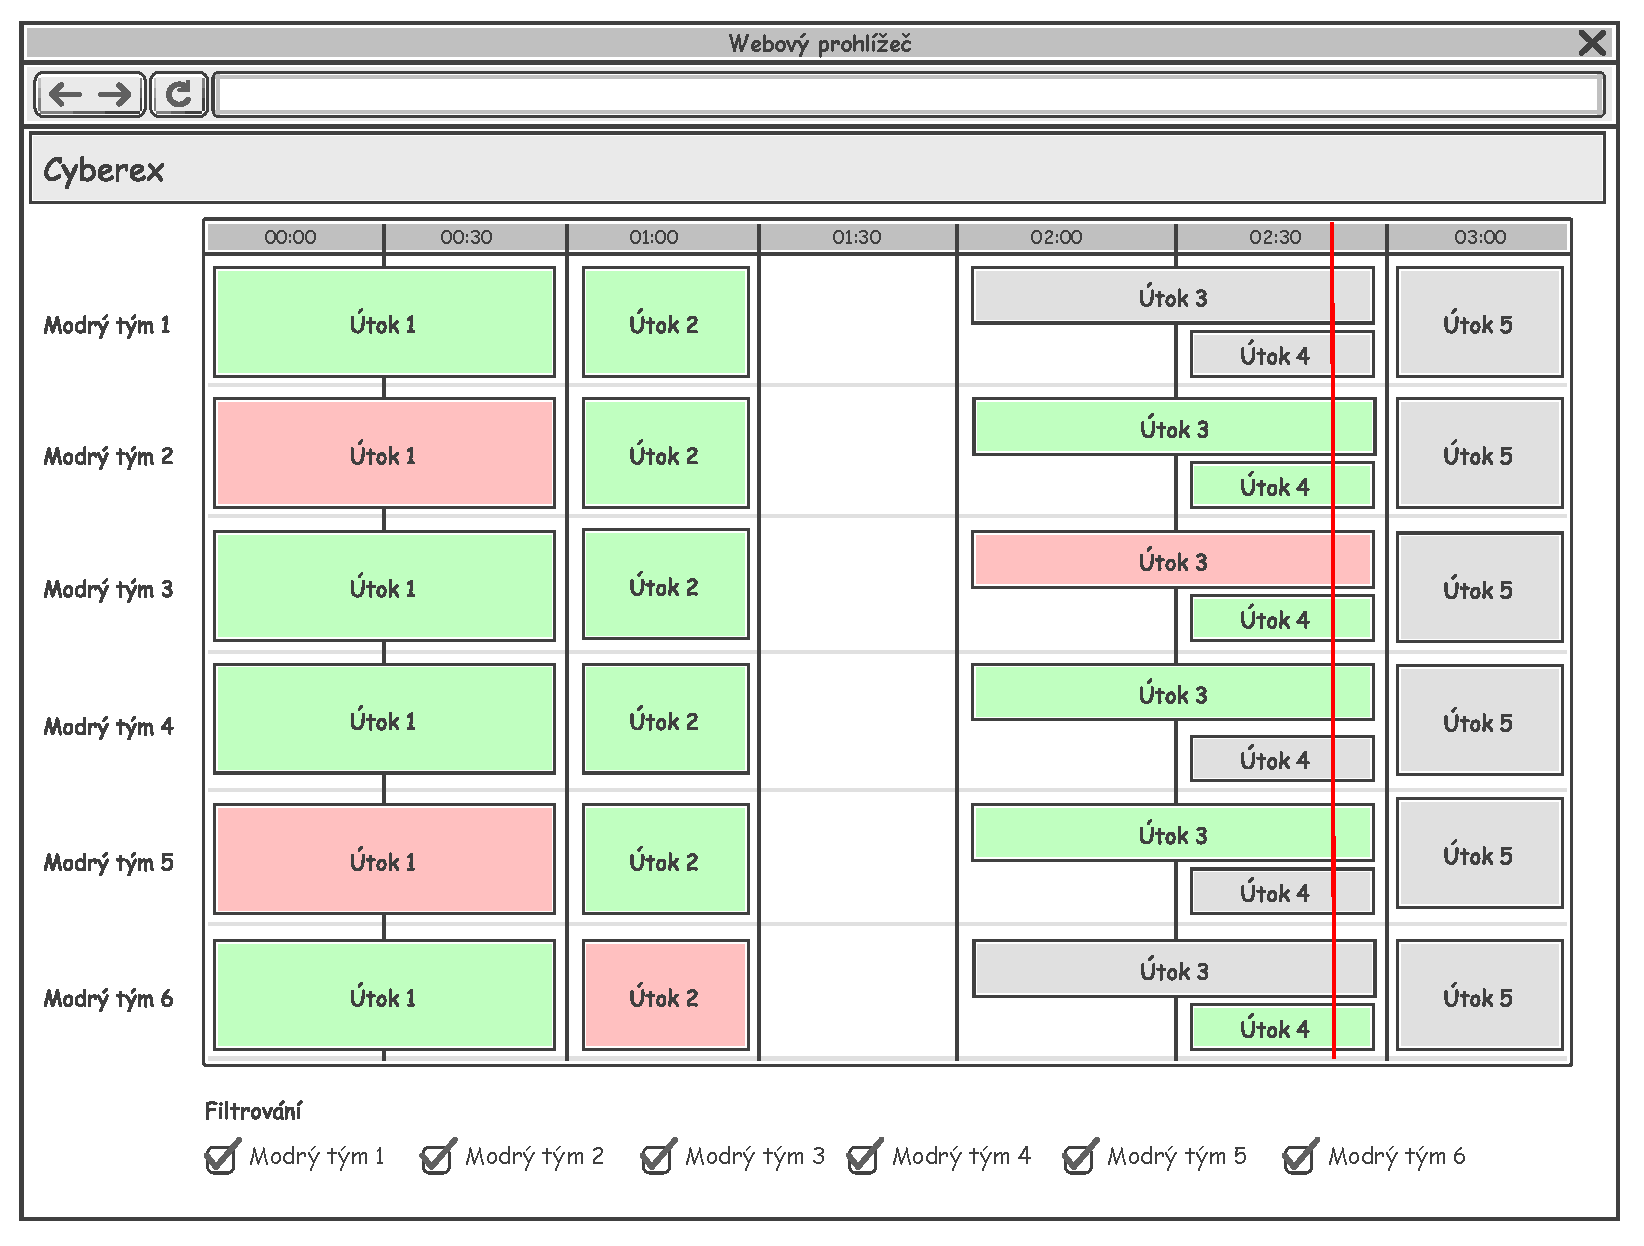
\includegraphics[width=13cm]{images/Web-Wireframe1.eps}
    \caption{Návrh znázorňující možnou podobu rozvrhu naplánovaných událostí v prezentační vrstvě. Události jsou zabarveny podle svého stavu. Zeleně jsou úspěšně dokončené události, červeně jsou neúspěšně dokončené události a šedě jsou události, které jsou, nebo budou prováděny. Svislá červená linka představuje aktuální čas na časové ose.}
    \label{fig:wireframeTimetable}
\end{figure}

Veškerou novou funkcionalitu systému zachycuje diagram případu užití na obrázku \ref{fig:useCase2}.

\begin{figure}
    \centering
    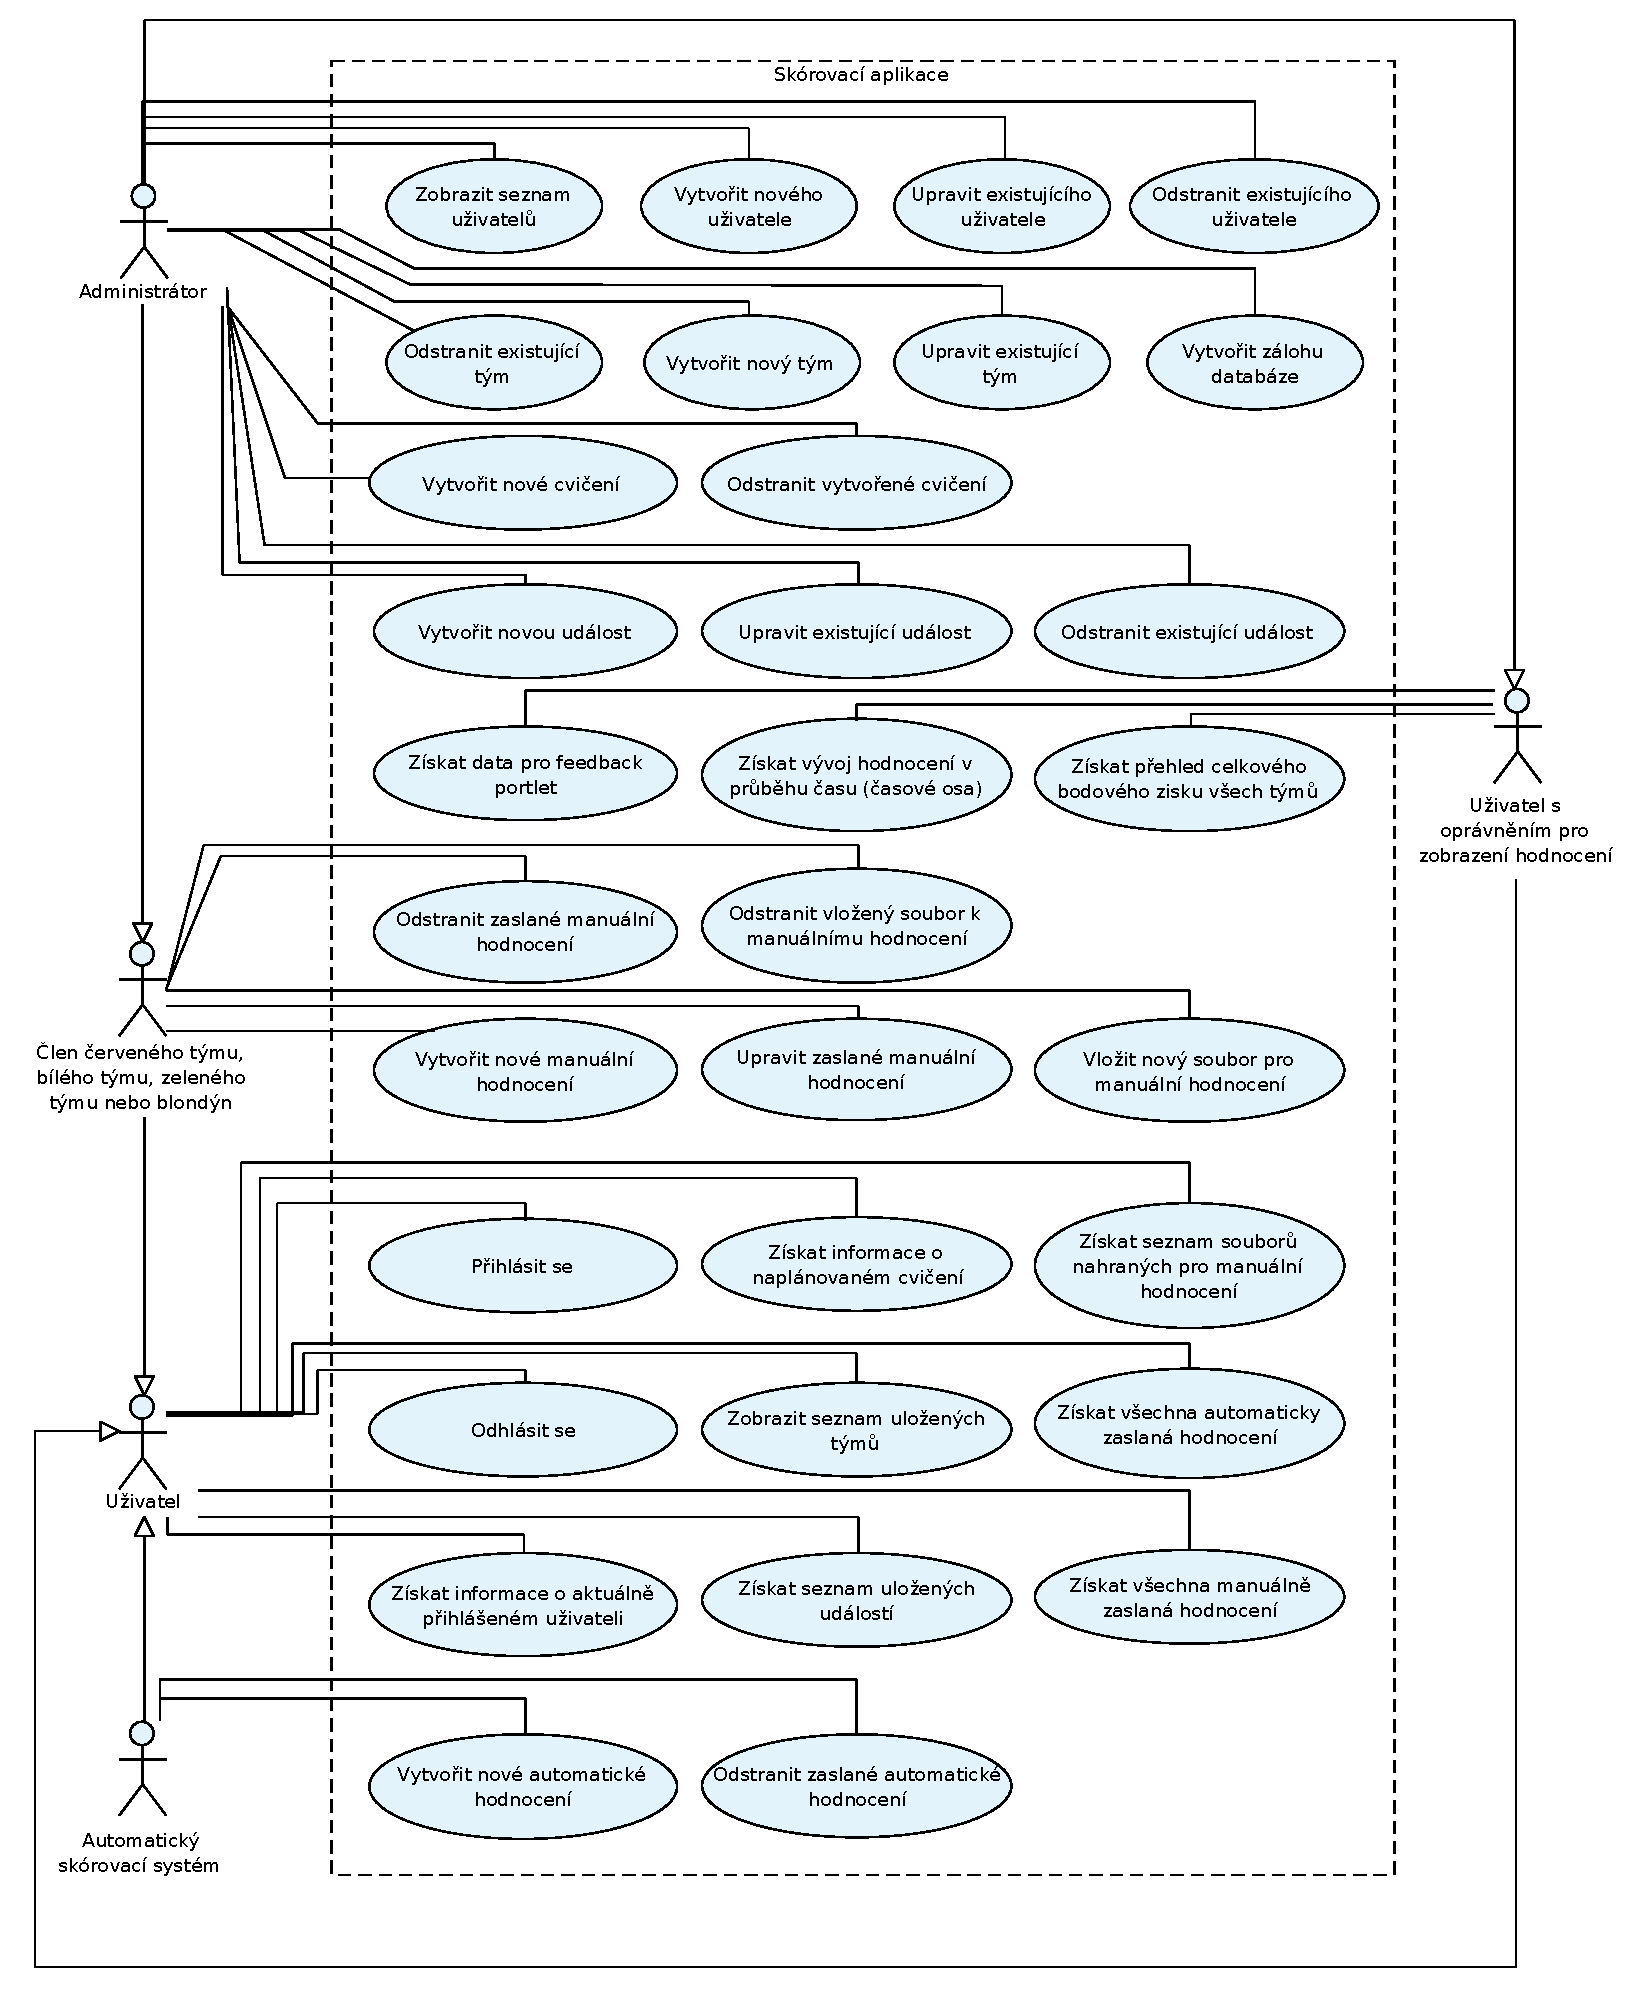
\includegraphics[width=15cm]{images/Use-case-2.eps}
    \caption{Diagram případu užití funkcionalit API nové hodnoticí aplikace.}
    \label{fig:useCase2}
\end{figure}

\section{Požadavky na použité technologie}

Původní hodnoticí aplikace byla implementována pomocí programovacího jazyka Python s~využitím frameworku Django. Tento systém velice usnadňuje tvorbu webových aplikací a~existuje pro něj rozšíření v~podobě Django REST framework. Rozšíření je určeno speciálně pro vytváření API a~pomocí nástrojů, které obsahuje, je možné efektivně vyvíjet propracované systémy. Výhodou tohoto frameworku je především výborná provázanost s~Django ORM systémem, kdy není nutné implementovat například funkce pro ukládání a~úpravu dat, protože tyto funkce jsou obstarány automaticky. Dále tato nástavba umožňuje snadný převod dat do strojově čitelných formátů (JSON, XML) za použití tzv. serializerů. Nezbytnou součástí frameworku je rozhraní pro vytváření automatických systémových testů pro jednotlivé přístupové body v~API.

U jazyka Python dojde k~přechodu z~verze 2.7 na verzi 3.5, aby bylo možné použít nejnovější vydání frameworku Django, který již Python 2.7 nepodporuje. Python 2.7 je již zastaralý a~bylo oznámeno ukončení podpory této verze k~roku 2020 \cite{python27}.


\section{Revize datového modelu}

Při revizi původního datového modelu jsem zjistil, že aplikace vykazuje mnohé nedostatky. Zaměřil jsem se především na odstranění duplicity dat a~kvalitnější interpretaci ukládaných informací, aby bylo možné sestavovat efektivnější databázové dotazy. Dále jsem se zabýval zlepšením v~oblasti řízení přístupu uživatelů k~datům.

Z pohledu duplicity dat bylo nevyhovující ukládání bodového hodnocení pro daný tým. Duplicita spočívala v~tom, že se při každém vložení nového hodnocení informace vložila nejprve do tabulky \texttt{logs} a~poté se aktualizovala hodnota se součtem hodnocení pro konkrétní tým v~tabulce \texttt{sumofobjectivelog}. Pro zápis jednoho hodnocení tedy bylo nutné vložit do databáze dva nové záznamy z~nichž jeden obsahoval duplicitní data.

V databázovém modelu chyběla identifikace uživatelů zodpovědných za vložený obsah nebo hodnocení. 

V případě ukládání manuálního a~automatického hodnocení se jedná o~data se stejnou strukturou. Bohužel, v~původním návrhu byla tato data ukládána odděleně do dvou tabulek \texttt{logs} a~\texttt{states}, což vedlo ke složitější logice při sestavování databázových dotazů.

\subsection{Návrh řešení nedostatků datového modelu}
Pro ukládání automatického nebo manuálního hodnocení je navržena jedna společná tabulka, která nese informaci o~tom, který tým je hodnocen, kdy bylo hodnocení provedeno a~počet udělených bodů. Data, která jsou specifická pro konkrétní typ hodnocení, jsou poté uložena v~samostatné tabulce. Mezi těmito tabulkami je vytvořena vazba. Díky tomu je možné snadněji procházet data pouze z~jednoho typu hodnocení.

Významnou změnou v~datovém modelu bylo vypuštění databázových tabulek, které obsahovaly průběžný součet bodů pro daný tým. Tyto tabulky bylo nutné aktualizovat při každé změně bodového hodnocení. Data o~aktuálním bodovém zisku daného týmu bude možné ukládat bez duplicit a~zjistit je i~bez původních tabulek pomocí agregačních dotazů nad tabulkou, ve které jsou uloženy veškeré záznamy z~hodnocení. Tato změna přinese zjednodušení ve výsledné implementaci aplikace.

Pro identifikaci, který uživatel je zodpovědný za zaslané hodnocení, případně další obsah, byl do tabulek \texttt{logs}, \texttt{files} a~\texttt{comments} přidán atribut pro uložení této informace. Nová aplikace bude využívat autentizačního a~autorizačního systému frameworku Django, z~tohoto důvodu je do tohoto atributu ukládán cizí klíč na tabulku \texttt{auth\_user}, která je součástí frameworku.

\subsection{Nový datový model}

Datový model samotné aplikace se skládá z~9 databázových tabulek. V~následující kapitole se budu zabývat podrobným popisem významu jednotlivých tabulek, definicí atributů a~popisu relačních vztahů.

\paragraph{Tabulka \texttt{exercises}} Ukládá informaci o~naplánovaném cvičení. V~tabulce je uložen čas začátku cvičení, délka trvání tohoto cvičení a~dále příznak, zda je záznam platný.

\paragraph{Tabulka \texttt{objectives}} Je využívána pro ukládání událostí, za které budou členové modrého týmu hodnoceni. Každá událost je tvořena názvem, zkratkou, volitelným popisem a~volitelnou fázi, která může být využita v~prezentační vrstvě pro seskupování událostí. Dále se v~tabulce nachází sloupce pro minimální a~maximální bodový rozsah, který je možné použít při zadávání hodnocení dané události a~každá událost má uloženou uživatelskou skupinu, která může danou událost hodnotit. Pro možnosti plánování a~vytváření rozvrhu událostí slouží sloupec pro uložení času od začátku cvičení, kdy má být událost (typicky útok) provedena a~sloupec určující, jak dlouho by událost měla probíhat. V~samotné aplikaci je ošetřeno, aby události s~nastaveným časem provedení nešly ohodnotit více než jedenkrát pro každý tým. Tímto je zajištěno, aby v~rozvrhu událostí bylo možné zobrazit, zda již byla daná událost provedena. 

\paragraph{Tabulka \texttt{teams}} Slouží pro ukládání informací o~modrých týmech. Každý tým musí mít unikátní název a~unikátní identifikátor v~prostředí KYPO, pomocí kterého bude možné párovat příchozí hodnocení z~automatického skórování. Pro každý tým lze nastavit příznak pro skrytí týmu v~tabulce s~hodnocením nebo lze volitelně nastavit vlajku a~barvu týmu, která bude využita v~prezentační vrstvě.

\paragraph{Tabulka \texttt{teamsJudges}} Reprezentuje vazbu M:N mezi tabulkami \texttt{teams} a~\texttt{auth\_users} a~umožňuje tak kontrolu, zda daný uživatel smí zadávat hodnocení pro daný tým. 

\paragraph{Tabulka \texttt{logs}} Představuje společné úložiště pro všechny příchozí druhy hodnocení. Každé hodnocení má společná data, a~to tým, kterému je hodnocení uděleno, dále čas udělení hodnocení, počet udělených bodů a~autora zaslaného hodnocení. Každý záznam v~této tabulce má nastaven příznak, který určuje, zda jde o~validní hodnocení, nebo hodnocení, které bylo smazáno. Ve sloupci \texttt{type} je uložena informace o~tom, o~jaký druh hodnocení se jedná. Rozlišení je provedeno pomocí numerických konstant zadefinovaných ve zdrojovém kódu aplikace.

\paragraph{Tabulka \texttt{automaticLogs}} Obsahuje záznamy o~zadaném automatickém hodnocení. Každý záznam má uloženou vazbu na záznam ve společné tabulce \texttt{logs}. Záznam v~tabulce \texttt{automaticLogs} nemůže existovat bez patřičného záznamu v~tabulce \texttt{logs}. Každé automatické hodnocení má uloženy informace o~zařízení, které bylo kontrolováno, o~službě, která byla kontrolována a~informaci o~stavu, v~jakém služba byla.

\paragraph{Tabulka \texttt{manualLogs}} Obsahuje naopak záznamy z~manuálně zadávaného hodnocení. Záznamy v~této tabulce opět nemohou existovat bez záznamu v~tabulce \texttt{logs}. Každé hodnocení má uloženou vazbu na danou událost v~tabulce \texttt{objectives} a~stav hodnocení, který určuje, zda byla událost provedena úspěšně, neúspěšně, případně  teprve čeká na provedení, nebo je právě prováděna. Tento stav se ukládá rovněž pomocí číselných konstant definovaných v~aplikaci.

\paragraph{Tabulka \texttt{files}} Slouží pro ukládání souborů k~zadanému hodnocení. Každý záznam má tedy referenci na patřičný záznam v~tabulce \texttt{logs}, cestu k~souboru, název souboru a~samotného autora souboru.

\paragraph{Tabulka \texttt{comments}} Je tabulka pro ukládání komentářů. Stejně jako soubory jsou vázány na konkrétní záznam v~tabulce \texttt{logs} a~je zde uložena reference na autora komentáře. Uvedené řešení umožňuje do budoucna rozšíření aplikace o~možnost diskuze více uživatelů nebo nahrávání souborů v~rámci jednoho hodnocení.

Zbývající tabulky \texttt{auth\_user}, \texttt{auth\_group} a~\texttt{auth\_user\_groups} jsou součástí Django frameworku a~v~modelu na obrázku \ref{fig:erdNewApp} níže jsou zaneseny pro znázornění, jak bylo tohoto autentizačního a~autorizačního systému, poskytovaného frameworkem, využito v~datovém modelu.

\begin{figure}
    \centering
    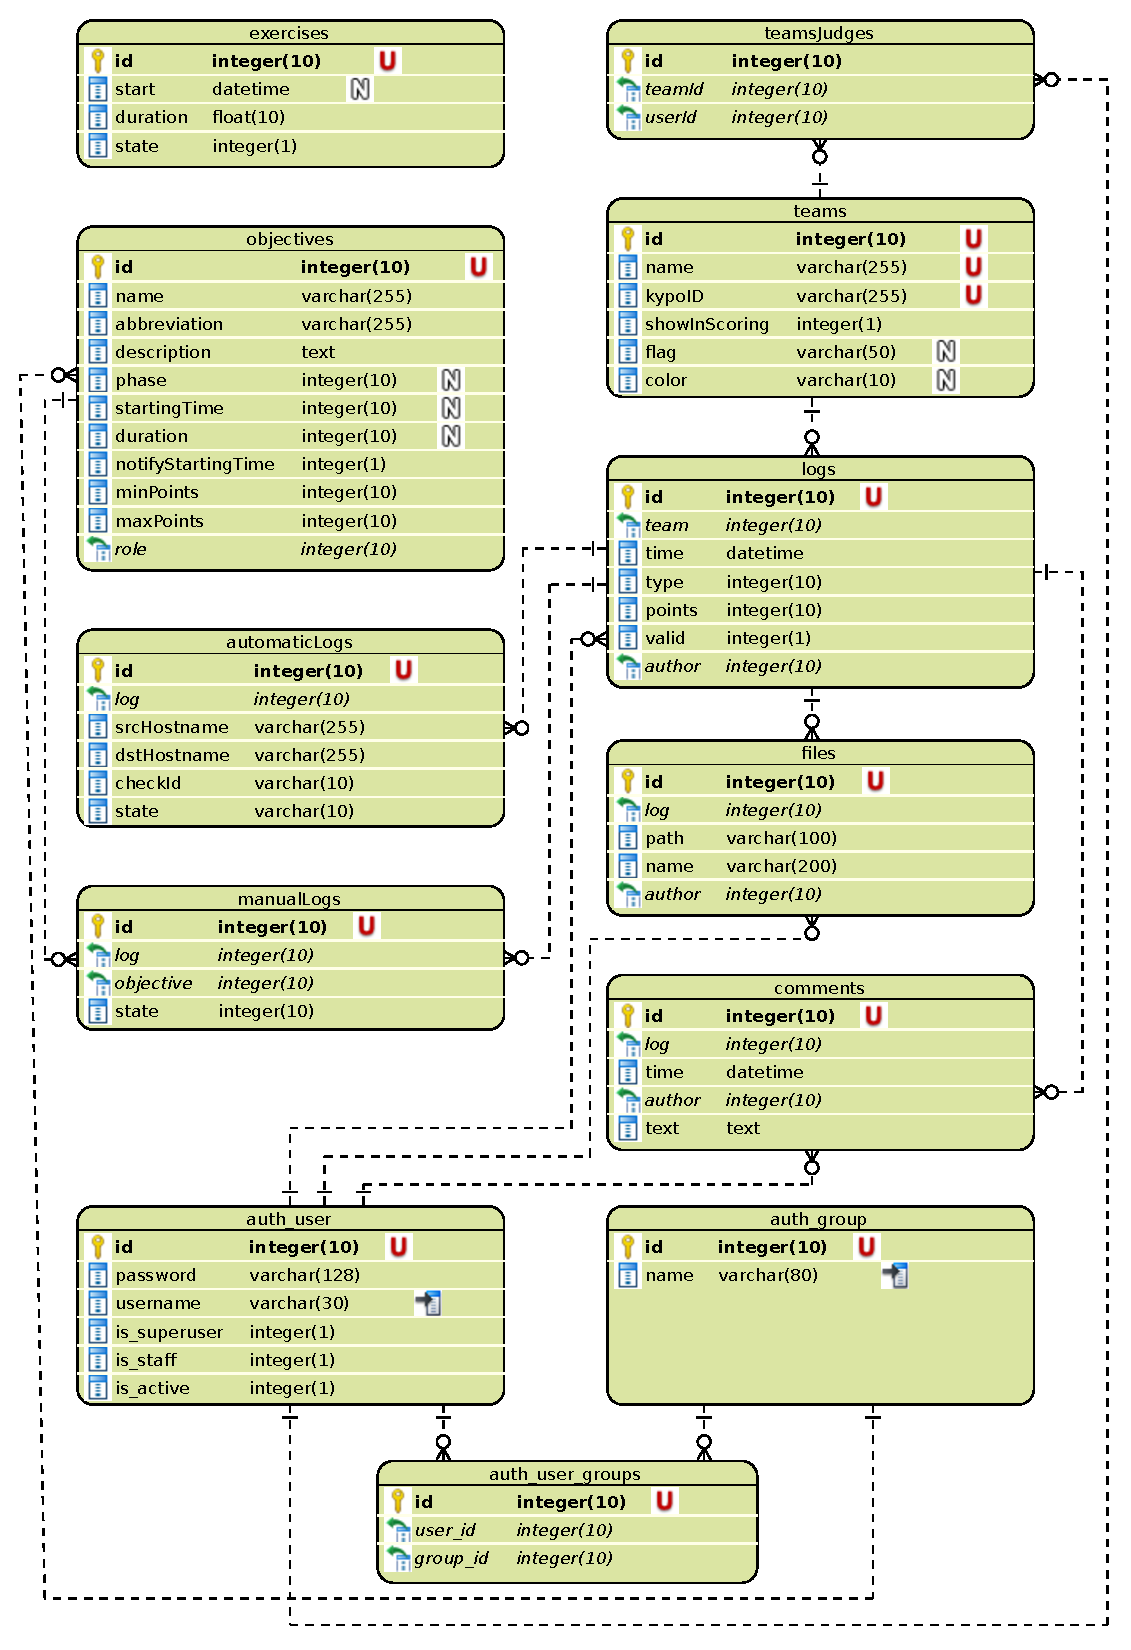
\includegraphics[width=12.5cm]{images/ERD-new-app.eps}
    \caption{Entitně relační diagram nového datového modelu.}
    \label{fig:erdNewApp}
\end{figure}

\newpage

\section{Návrh API}

Po dokončení revize datového modelu byl vytvořen návrh API pro novou aplikaci. Tento návrh se řídil principy REST (Representational State Transfer), což je softwarová architektura, definující sadu pravidel, jakým způsobem bude přistupováno k~určitému webovému zdroji a~jakým způsobem budou probíhat operace s~tímto zdrojem \cite{RoyThomasFielding2000ArchitecturalArchitectures}.
REST architektura byla navržena pro distribuované systémy, ve kterých jsou komponenty systému rozděleny do samostatných celků komunikujících pomocí zasílání zpráv přes počítačovou síť. V~našem případě je toto prostředí představováno oddělenou servisní a~prezentační vrstvou a~pro komunikaci je využit HTTP protokol.  Dle principů REST by webový zdroj měl podporovat operaci čtení, vytváření, upravování a~mazání, tedy tzv. CRUD\footnote{Zkratka shrnující čtyři základní operace s~daty. Vytvoření (create), čtení (read), úprava (update) a~mazání (delete).}. V~případě HTTP protokolu se využívá metody GET pro získání dat, POST pro vytváření dat, PUT pro úpravu již existujících dat a~DELETE pro mazání dat. Dále tato architektura popisuje, jakým způsobem by měla být data reprezentována ve strojově čitelném formátu. \cite{RoyThomasFielding2000ArchitecturalArchitectures}

Při návrhu API jsem využil online nástroje Swagger \cite{swagger}, který generuje velice přehlednou dokumentaci pro API a~umožňuje její sdílení i~dalším vývojářům. V~příloze \ref{appendAPI} se nachází stručný přehled struktury API. Kompletní dokumentace s~přesným popisem odesílaných a~přijímaných dat se nachází v~elektronických přílohách práce.

\chapter{Implementace nové hodnoticí aplikace}
\label{implementationNewApp}

\section{Struktura projektu}
Pro implementaci byl využit Framework Django ve spojení s~Django REST framework. Díky zvoleným nástrojům lze vytvářet přehledný a~strukturovaný kód. V~následujících kapitolách popíšu nejdůležitější části struktury nově vytvořené aplikace.

\subsection{Řadič}
\label{radic}
Všechny příchozí požadavky na webserver jsou předány do Django aplikace a pomocí routovacích pravidel jsou předány patřičným funkcím, které představují řídící logiku celé aplikace. V~případě příchozích požadavků na získání informací funkce provede načtení dat z~modelu. Následuje předání dat do serializační metody a~vzniklý výstup je odeslán v~odpovědi serveru. Funkce zajišťuje při požadavcích na vytváření, úpravu nebo mazání záznamů předání přijatých dat do serializační metody. V~případě validační chyby dat se funkce postará o~vygenerování chybového hlášení. Pokud je nový záznam úspěšně vytvořen nebo upraven, odešle funkce v~odpovědi serveru tento záznam.

\subsection{Model}
\label{model}
Framework Django obsahuje propracovaný ORM systém. Veškeré datové modely jsou popsány univerzálním popisem datové struktury a~na základě těchto definic je automaticky vygenerována struktura databáze. ORM systém je nezávislý na použitém databázovém systému. Podporované databázové systémy jsou PostgreSQL, MySQL, SQLite a~Oracle. Framework sám spravuje schéma databáze a~sestavuje dotazy podle zvoleného databázového systému.

Každá entita je reprezentována samostatnou třídou a~může být rozšířena o~vlastní metody. Uvedený přístup byl vhodný například při implementaci funkce, která získá pro entitu týmu všechna vložená hodnocení. Tímto je zachována lepší strukturu kódu, jelikož metody, které se starají pouze o~získání dat, jsou stále zapsány v~modelu.

\subsection{Serializace dat}
\label{serializer}
V systému jsou databázová data reprezentována pomocí entit ORM systému, pro jejich převod do strojově čitelného formátu slouží speciální serializační třídy. Pomocí těchto tříd lze však provést i~opačný proces, tedy ze strojově čitelného formátu vytvořit nebo upravit entitu. Pomocí mapování na ORM datový model je možné realizovat, aby tento proces probíhal zcela automaticky. Programátor však může i~nadále do tohoto procesu zasáhnout implementací vlastní metody pro ukládání či editaci. Implementace vlastních metod jsem využil pro ukládání záznamu o~hodnocení, kdy se ukládají data do dvou různých databázových tabulek a~není tak možné využít generického chování funkcí pro ukládání.

\subsection{Adresářová struktura}
V hlavním adresáři aplikace se nachází soubor \texttt{manage.py}. Soubor slouží pro spouštění příkazů frameworku Django, tedy například spuštění vývojového webového serveru nebo automatických testů. Adresářová struktura je rozdělena na dva samostatné adresáře \texttt{scoring} a~\texttt{cyberex\_api}.

Adresář \texttt{scoring} obsahuje konfigurační soubor \texttt{settings.py}, ve kterém se nachází veškeré nastavení aplikace. V~souboru \texttt{globals.py} je zadefinována hodnota výchozího bodového skóre každého týmu. Soubor \texttt{urls.py} obsahuje routovací pravidla, pomocí kterých se příchozí požadavky předávají jednotlivým modulům, respektive funkcím.

Příchozí požadavky na webserver jsou dle modulů rozděleny podle následujícího přehledu.

\begin{itemize}
    \item \texttt{api/v1/} -- modul hodnoticí aplikace
    \item \texttt{api\-auth/v1/} -- modul zajišťující autentizaci
    \item \texttt{admin/} -- modul administrace, která je generována frameworkem
\end{itemize}

Adresář \texttt{cyberex\_api} obsahuje veškeré zdrojové kódy hodnoticí aplikace. Adresářová struktura je následující.

\begin{itemize}
    \item \texttt{admin.py} -- konfigurace pro automaticky generovanou administraci
    \item \texttt{helpers.py} -- pomocné funkce, např. pro počítání herního času k~záznamům o~hodnocení
    \item \texttt{models.py} -- definice databázového modelu pro ORM systém, viz kapitola \ref{model}
    \item \texttt{permissions.py} -- pravidla autorizačního systému
    \item \texttt{serializers.py} -- soubor tříd zajišťující převod dat do strojově čitelného formátu, viz kapitola \ref{serializer}
    \item \texttt{tests.py} -- automatické testy, viz kapitola \ref{testovani}
    \item \texttt{urls.py} -- definice routovacích pravidel, na základě příchozího požadavku je každý požadavek předán správné funkci v~souboru \texttt{views.py}
    \item \texttt{views.py} -- soubor tříd, které obsluhují příchozí požadavky, viz kapitola \ref{radic}
\end{itemize}

\section{Automatické testování}
\label{testovani}
Nedílnou součástí celého projektu jsou automatické systémové testy, které testují aplikaci jako celek, zda se chová dle požadavků \cite{difSysTest}.

Díky svojí komplexitě mohou testy odhalit chybné chování na kterékoliv vrstvě aplikace. Příkladem systémového testu je vložení nového záznamu do systému pomocí API a~následné provedení kontroly, zda odpověď serveru obsahuje očekávaná data včetně kontroly správného uložení dat v~databázovém systému.

Pro implementaci testů byly využity knihovny obsažené v~Django REST framework. Pomocí dostupných funkcí je možné sestavit HTTP požadavek, který bude odeslán na spuštěný vývojový server. Po odeslání požadavku je možné provést kontrolu, zda data obdržená v~odpovědi serveru odpovídají očekávaným datům. V~případě vytváření, úpravy nebo mazání dat se zároveň provádí i~kontrola dat v~databázovém systému. 

Celkem bylo implementováno 57 testů. Pro každý existující koncový bod API a~každou dostupnou HTTP metodu existuje minimálně jeden test. Pro metody POST a~PUT existují typicky varianty testu s~validními a~nevalidními daty. Testy se nachází v~souboru \texttt{tests.py} v~adresáři \texttt{cyberex\_api} a~jejich spuštění je možné provést v~příkazové řádce spuštěním příkazu \texttt{test} frameworku Django.

Výše uvedené testy jsem využíval pro ověření funkčnosti celého systému po provedení úprav. V~praxi je vhodné ověřovat testováním funkčnost softwaru před každou změnou na produkčním prostředí.

\section{Instalace a~spouštění aplikace}
Aplikace pro svůj běh vyžaduje interpretr jazyka Python ve verzi 3.5 a~instalaci několika dalších modulů. Abych zajistil co nejjednodušší instalaci těchto závislostí, rozhodl jsem se využít nástroje Pipenv \cite{pipenv}. V~následujících kapitolách popíšu použití tohoto nástroje a~způsob, jakým byla aplikace distribuována mezi další vývojáře.

\subsection{Řešení závislostí pomocí nástroje Pipenv}
Nástroj Pipenv v~sobě spojuje dvě důležité funkcionality. První je správce balíčků, pomocí kterého je možné snadno definovat všechny potřebné závislosti aplikace a~následně je jednorázově nainstalovat jediným příkazem. Druhou funkcionalitou je nástroj pro spouštění softwaru v~uzavřeném prostředí, které je nakonfigurováno podle definovaných závislostí. Díky tomu je možné v~jednom operačním systému spouštět programy pro rozdílné verze jazyka Python a~odlišné verze modulů tohoto jazyka.

Veškeré závislosti jsou definovány v~souboru \texttt{Pipfile}, kde se nachází požadovaná verze jazyka Python a~seznam vyžadovaných modulů. Pro spuštění je nutné mít na počítači nainstalován interpreter jazyka Python a~nástroj Pipenv. Pomocí příkazu programu Pipenv lze nainstalovat veškeré závislosti.

\begin{lstlisting}
pipenv install
\end{lstlisting}

\noindent
Pomocí dalšího příkazu lze již spustit samotnou aplikaci.

\begin{lstlisting}
pipenv run runserver
\end{lstlisting}

Příkaz \lstinline[columns=fixed]{pipenv run runserver} je alias definovaný v~souboru \texttt{Pipfile} a~reprezentuje příkaz \lstinline[columns=fixed]{python manage.py runserver}. Příkaz zapne vývojový server frameworku Django.

Díky použitým nástrojům je spuštění aplikace velice snadné, ale je zde několik dalších nedostatků. Instalace se skládá z~několika kroků, při kterých může dojít k~chybě. V~nainstalované aplikaci neexistují žádná testovací data, včetně uživatelských účtů a~vývojový server, spouštěný při lokální instalaci, se liší od serveru, který je používán v~produkčním prostředí v~KYPO. Z~těchto důvodů jsem se rozhodl pro využití nástroje Vagrant \cite{vagrant}, který za pomocí virtualizace spustí a~nakonfiguruje nový virtuální počítač s hodnoticí aplikací.

\subsection{Spuštění aplikace ve virtuálním prostředí}

Pro zprovoznění aplikace je nezbytné mít k~dispozici počítač podporující virtualizaci a~dále nainstalované programy VirtualBox \cite{virtualbox} a~Vagrant. Pomocí jediného příkazu poté dojde ke spuštění virtuálního počítače, na který bude předinstalován operační systém Linux a~do tohoto systému budou následně nainstalovány veškeré programy a~balíčky nutné pro fungování aplikace. Po připravení prostředí pro běh systému jsou spuštěny další příkazy, které provedou vytvoření uživatelských účtů a~testovacích dat, aby bylo možné spuštěnou aplikaci ihned využívat. 

Prostředí ve virtuálním počítači je nakonfigurováno tak, aby se co nejvíce blížilo produkčnímu prostředí v~KYPO. Jako webový server se používá Apache2, který je nakonfigurován tak, aby komunikoval pomocí šifrovaného protokolu HTTPS. Aplikace s~webovým serverem komunikuje pomocí WSGI (Web Server Gateway Interface). WSGI představuje jednotné rozhraní pro komunikaci webových serverů a~aplikací naprogramovaných v~jazyce Python.

Jako relační databázový systém se využívá SQLite, který byl zvolen převážně kvůli svojí jednoduchosti.

\section{Reálné nasazení aplikace}

Vytvořená aplikace byla použita při dvou cvičeních Cyber Czech 2018, která se konala v termínech 16.--17. října a 20.--21. listopadu. Před samotným cvičením Cyber Czech proběhly ještě dvě generální zkoušky v termínech 21. září a 12. října. V následujících kapitolách popíšu jednotlivé použití aplikace a zjištěné nedostatky.

\subsection{Generální zkoušky}
Při generálních zkouškách byla testována funkčnost servisní vrstvy hodnoticí aplikace spolu s prezentační vrstvou. Oba systémy spolu bez problému spolupracovaly a nebyl objeven žádný problém v propojení těchto systémů. Poprvé byla vyzkoušena hodnoticí aplikace na širším okruhu uživatelů. Ve webové aplikaci se během zkoušky objevily drobné nedostatky, avšak i přesto sklidila aplikace pozitivní hodnocení.

Drobné problémy byly objeveny i v servisní vrstvě aplikace. Některé koncové body API měly příliš vysokou odezvu, a~bylo proto nutné provést jejich optimalizaci.

Aplikace získává při volání koncového bodu \texttt{/charts/score} v~API aktuální výsledky bodů z~automatického skórování nad tabulkou \texttt{logs}. Během jednoho cvičení může být vygenerováno až 10 000 záznamů hodnocení, a~tak aplikace musí být schopna pracovat s~velkými počty záznamů. Testováním aplikace se ukázalo, že ORM systém je pro operace nad tímto množstvím dat nevhodný a~získávání skóre trvalo řádově několik sekund. V~tomto případě se ukázalo jako efektivní využít agregačních SQL dotazů. 

Konkrétně byl pro získání celkového bodového zisku z~automatického skórování použit následující SQL dotaz.

\begin{markdown*}{%
  fencedCode,
}
```
SELECT team_id, SUM(points) FROM logs 
WHERE type = 2 AND valid = 1 
GROUP BY team_id
```
\end{markdown*}

Dotaz využívá funkce \texttt{SUM} pro získání součtu bodů a~klauzule \texttt{GROUP\ BY} pro seskupení dat podle identifikátorů jednotlivých týmů. Výběr dat je omezen pouze na validní záznamy z~automatického skórování.

Všechny změny bodového skóre v~čase se získávají pomocí volání API \texttt{/charts/timeline}. Vzhledem k~tomu, že tyto hodnoty se opět berou z~výše uvedené tabulky \texttt{logs}, naráží tato operace opět na limity ORM systému. S~přihlédnutím ke skutečnosti, že automatický skórovací systém vkládá do aplikace záznamy o~nedostupnosti služeb v~dávkách (např. 4 záznamy ve stejný okamžik), jsem se rozhodl využít opět agregační dotaz, který takové záznamy spojí do jednoho a~zrychlí tak získávání záznamů a~sníží se datový objem dat.

\noindent
Výsledný SQL dotaz má nasledující podobu.

\begin{markdown*}{%
  fencedCode,
}
```
SELECT team_id, time, SUM(points) FROM logs 
WHERE valid = 1 
GROUP BY strftime('%s', time), team_id 
ORDER BY time
```
\end{markdown*}

V dotazu dochází pomocí klauzule \texttt{GROUP\ BY} k~seskupení dat, která mají stejný čas vložení. Opět je využito funkce \texttt{SUM} pro získání celkové sumy bodů.

Díky těmto úpravám došlo ke snížení odezvy těchto koncových bodů API z~několika sekund na řádově stovky milisekund. 

\subsection{První běh cvičení}

Jelikož v~prezentační vrstvě nebyla dosud implementována správa uživatelů, bylo nutné před samotným cvičením aktivovat v~aplikaci automatickou administraci frameworku Django. Kromě správy uživatelů jsem v~administraci povolil přístup i~ke správě týmů a~veškerého hodnocení. Účelem tohoto nástroje se stalo umožnit servisní zásah do celé aplikace, při běžném používání však není tento nástroj potřebný. Administrace je mimo jiné využívána i~pro vymazání veškerého obsahu z~databáze před zahájením nového cvičení.

Při prvním cvičení se objevil jediný problém. Spočíval v~tom, že vlivem neznámé chyby se v~administraci aplikace nezobrazilo několik záznamů z~manuálního hodnocení, vložených při předchozím testování. Při mazání všech záznamů zůstalo toto hodnocení uloženo v~tabulce \texttt{manualLogs}. Získávání seznamu manuálního hodnocení v~API tyto záznamy neodesílalo, jelikož k~nim neexistoval žádný záznam v~tabulce \texttt{logs}. Během cvičení však v~tabulce \texttt{logs} vznikly nové záznamy z~automatického hodnocení a~tyto měly identifikátory shodné s~těmi, které byly uloženy u~nezobrazeného hodnocení. Kvůli existenci záznamů v~tabulce \texttt{logs} se začaly neviditelné manuální hodnocení zobrazovat, a~bylo tak nutné je manuálně smazat. Abych v~budoucnu podobné situace předešel, doplnil jsem software o~modul SQL Explorer \cite{sqlexplorer}, pomocí kterého je umožněno administrátorovi spouštět databázové dotazy, a~je tak možné odhalit případnou chybu v~databázi.

\subsection{Druhý běh cvičení}
Během druhého cvičení se objevily problémy s~odezvou API, které však byly způsobeny dlouhodobým přetížením serveru, kde byla aplikace spuštěna. Dále se ukázalo, že aplikace stále nedisponuje dostatkem nástrojů pro případ nutného servisního zásahu. Při cvičení se objevila chyba v~jednom ze systémů, se kterým pracovali členové modrého týmu. Vlivem této chyby došlo k~vložení několika stovek automatických hodnocení, které bylo potřeba smazat. Nástroj SQL Explorer, který jsem přidal po prvním cvičení, umožňoval přístup k~datům pouze v~režimu pro čtení a~veškeré neplatné záznamy bylo nutné smazat manuálně. Po tomto cvičení jsem nástroj upravil, aby umožňoval použití i~modifikačních SQL dotazů a~do budoucna je pro administrátora zajištěn plnohodnotný nástroj pro jakýkoliv zásah do databáze.

\chapter{Závěr}
\label{end}

V rámci mojí bakalářské práce jsem provedl rozbor stávající hodnoticí aplikace a~na základě zjištěných nedostatků jsem vytvořil návrh datového modelu a~aplikačního programového rozhraní pro novou aplikaci, kterou jsem následně implementoval za použití Django REST Framework. Vytvořený nástroj zajišťuje servisní vrstvu celé hodnoticí aplikace a~pomocí REST API komunikuje s~prezentační vrstvou, která je vytvořena jako webová aplikace a~vznikla v~rámci jiné bakalářské práce. 

Jako celek tento vytvořený software plně nahradil stávající aplikaci a~kromě zachování veškeré původní funkcionality byl také nástroj rozšířen o~nové funkce, které uživatelům aplikace umožní komfortnější používání a~organizátorům cvičení zajistí možnost lepšího řízení celého cvičení. Jedná se například o~možnost zobrazení rozvrhu s~naplánovanými událostmi nebo zlepšení správy uživatelských účtů viz kapitola \ref{novePozadavky}.

Díky reálnému využití je jisté, že v~budoucnu se bude aplikace dále rozšiřovat o~nové funkce, a~proto pro mě při vývoji bylo prioritou vytvoření přehledného kódu, který bude vhodně rozvržen do samostatných metod a~bude respektovat principy MVC (Model-view-controller) architektury. Implementace nových funkcí tak bude mnohem snazší. Velký důraz jsem kladl i~na vytvoření dostatečného množství automatických testů, aby bylo možné kdykoliv ověřit funkčnost celé aplikace.

Během vývoje jsem se setkal s~technologiemi, které pro mě byly zcela nové a~práce pro mě byla o~to zajímavější. S~postupným získáváním znalostí jsem některé části aplikace refaktoroval, až jsem docílil stavu, se kterým jsem byl plně spokojen. Odměnou pro mě bylo, že aplikace během obou cvičení nevykazovala žádné chyby v~mnou implementovaných částech a~od uživatelů přicházely na hodnoticí aplikaci pozitivní ohlasy.

Po druhém použití v praxi se objevily nápady, jak aplikaci rozšířit. Užitečnou funkcí, která by ulehčila přípravu aplikace na nové cvičení, by byla možnost hromadného vymazání záznamů o hodnocení, pokud právě neprobíhá žádné cvičení. Pro tuto funkci by mohl existovat nový koncový bod v~API, který by mohl spustit pouze administrátor. 

Další užitečnou funkcí, kterou by aplikace mohla disponovat, je výpis všech služeb, které jsou kontrolovány automatickým skórováním, a~to včetně stavu těchto služeb. Výpis by obsahoval názvy služeb, barevně by byl odlišen stav dostupnosti každé služby a mohla by být zobrazena informace o tom, kolik celkem bylo za nedostupnost dané služby strženo bodů.

Výpisu by mohlo být využito pro porovnávání aktuálního stavu mezi všemi týmy a mohl by být i veřejně prezentován pro ukázání rozdílů mezi týmy. Funkce, která by mohla přinést zjednodušení v~práci s~aplikací, je propojení správy uživatelů s~již existujícím systémem v~KYPO. Uživatelské účty jsou zvlášť vytvářeny v hodnoticí aplikaci a~zvlášť v~portálu KYPO, který slouží pro přístup ke všem ostatním systémům používaným při cvičení. Pokud by do budoucna bylo možné tyto přihlašovací procesy spojit, přineslo by to zjednodušení celé správy uživatelů. Obdobný námět na vylepšení platí i~pro správu týmů, které jsou opět zadávány do portálu KYPO a~samostatně do hodnoticí aplikace. Pro správné spárování týmů je v hodnoticí aplikaci uložen identifikátor týmu z~portálu KYPO.

\printbibliography[heading=bibintoc] %% Print the bibliography.

\appendix %% Start the appendices.
\chapter{Informace k elektronické příloze}

Elektronická příloha obsahuje dva adresáře.

\paragraph{Dokumentace API} Adresář obsahuje soubor \texttt{index.html}, který lze otevřít ve webovém prohlížeči a obsahuje offline dokumentaci API. Online dokumentace je dostupná na adrese \url{https://app.swaggerhub.com/apis/muni-cyberex/Cyberex_control_app/1.0.0#/}.
    
\paragraph{cyberex-control-app} Adresář obsahuje zdrojové kódy aplikace. Pro spuštění aplikace je nutné mít nainstalován program VirtualBox verze 5 nebo vyšší a Vagrant verze 1.9 nebo vyšší.
\begin{itemize}
    \item \url{https://www.virtualbox.org/wiki/Downloads}
    \item \url{https://www.vagrantup.com/downloads.html}
\end{itemize}
Pro spuštění stačí v adresáři \texttt{cyberex-control-app} spustit příkaz \texttt{vagrant up}.
Po úspěšném spuštění virtuálního počítače bude aplikace dostupná na adrese
\texttt{192.168.88.99} pomocí protokolu \texttt{HTTPS}. V případě kolize této adresy s jinou adresou v síti je nutné
před spuštěním virtuálního stroje upravit tuto adresu v souboru \texttt{Vagrantfile}.
Do virtuálního počítače bude nainstalován operační systém Ubuntu 16.04.
Minimální požadavky na virtuální počítač, ve kterém bude aplikace spuštěna,
jsou:
\begin{itemize}
    \item RAM 1024 MB
    \item HDD 5 GB
    \item 900 MHz x86 procesor
\end{itemize}
Soubor \texttt{README.md} v adresáři \texttt{cyberex-control-app} obsahuje veškeré informace o tom, jak provést spuštění aplikace, jak provést přihlášení do aplikace a následně odeslat testovací požadavek do API.

\chapter{Struktura API nové hodnoticí aplikace}
\label{appendAPI}

\renewcommand\labelitemii{$\square$}
\begin{itemize}
    \item \texttt{/users}
    \begin{itemize}
        \item \texttt{GET} -- získání seznamu všech uživatelů
        \item \texttt{POST} --  vytvoření nového uživatele
    \end{itemize}
    
    \item \texttt{/users/\{user\}}
    \begin{itemize}
        \item \texttt{GET} -- získání detailu uživatele
        \item \texttt{PUT} -- upravení existujícího uživatele
        \item \texttt{DELETE} -- odstranění existujícího uživatele
    \end{itemize}
    
    \item \texttt{/teams}
    \begin{itemize}
        \item \texttt{GET} -- získání seznamu všech týmů
        \item \texttt{POST} --  vytvoření nového týmu
    \end{itemize}
    
    \item \texttt{/teams/\{team\}}
    \begin{itemize}
        \item \texttt{GET} -- získání detailu týmu
        \item \texttt{PUT} -- upravení existujícího týmu
        \item \texttt{DELETE} -- odstranění existujícího týmu
    \end{itemize}
    
    \item \texttt{/exercises}
    \begin{itemize}
        \item \texttt{GET} -- získání informací o~naplánovaném cvičení
        \item \texttt{POST} -- vytvoření nového cvičení
    \end{itemize}
    
    \item \texttt{/objectives}
    \begin{itemize}
        \item \texttt{GET} -- získání seznam všech událostí
        \item \texttt{POST} --  vytvoření nové události
    \end{itemize}
        
    \item \texttt{/objectives/\{objective\}}
    \begin{itemize}
        \item \texttt{GET} -- získání detailu události
        \item \texttt{PUT} -- upravení existující události
        \item \texttt{DELETE} -- odstranění existující události
    \end{itemize}
        
    \item \texttt{/charts/timeline}
    \begin{itemize}
        \item \texttt{GET} -- získání časové osy s~jednotlivými změnami bodového hodnocení
    \end{itemize}
        
    \item \texttt{/charts/score}
    \begin{itemize}
        \item \texttt{GET} -- získání celkového skóre
    \end{itemize}
        
    \item \texttt{/logs/automatic}
    \begin{itemize}
        \item \texttt{GET} -- získání seznamu všech automatických hodnocení
        \item \texttt{POST} --  vytvoření nového automatického hodnocení
    \end{itemize}
        
    \item \texttt{/logs/automatic/\{log\}}
    \begin{itemize}
        \item \texttt{GET} -- získání detailu automatického hodnocení
        \item \texttt{DELETE} -- odstranění existující události
    \end{itemize}
            
    \item \texttt{/logs/manual}
    \begin{itemize}
        \item \texttt{GET} -- získání seznamu všech manuálních hodnocení
        \item \texttt{POST} --  vytvoření nového manuálního hodnocení
    \end{itemize}
            
    \item \texttt{/logs/manual/\{log\}}
    \begin{itemize}
        \item \texttt{GET} -- získání detailu manuálního hodnocení
        \item \texttt{PUT} -- upravení existujícího hodnocení
        \item \texttt{DELETE} -- odstranění existujícího hodnocení
    \end{itemize}
            
    \item \texttt{/logs/manual/\{log\}/files}
    \begin{itemize}
        \item \texttt{GET} -- získání seznamu všech souborů pro dané manuálních hodnocení
        \item \texttt{POST} -- vytvoření nového souboru pro dané hodnocení
    \end{itemize}
            
    \item \texttt{/logs/manual/\{log\}/files/\{file\}}
    \begin{itemize}
        \item \texttt{DELETE} -- odstranění existujícího souboru
    \end{itemize}
            
    \item \texttt{/export/database}
    \begin{itemize}
        \item \texttt{GET} -- získání odkazu pro stažení zálohy databáze
    \end{itemize}
                
    \item \texttt{/export/feedback}
    \begin{itemize}
        \item \texttt{GET} -- získání dat pro feedback portlet (slouží pro přípravu dokumentů se zpětnou vazbou pro členy modrého týmu)
    \end{itemize}

\end{itemize}

\end{document}